%!TEX root = MemoireZelliges.tex

\chapter{Étude physique d'un zellige bleu verdâtre (\bdx{6529})}
%======================================================================

\section{Description -- État de surface}
%----------------------------------------------------------------------

Il s'agit d'un zellige provenant du \PaM, \siecle{17}, (Meknès, 
Maroc). De forme parallélépipédique, il comporte une glaçure bleu vert 
(\fref{dessin:6529}). Beaucoup plus épais et plus grand que les quatre 
autres échantillons, il est aussi le seul à ne pas être chanfreiné. 
On remarque également des coulures de la glaçure sur ses bords. Les 
traces d'encre sont dues à l'indexation de l'échantillon au Maroc.

Il s'agirait en fait, non pas d'un élément du décor de zelliges, mais 
plutôt d'un carreau utilisé pour le cerner. La présence de coulures 
indique que l'échantillon n'a pas subi de découpe après cuisson et 
leur répartition homogène sur ses quatre faces montre qu'il a été cuit 
à plat.

\begin{itemize}
  \item \DimText : \SI{75x59x39}{\mm}
  \item \emph{Masse} : \SI{257.1}{\g}
\end{itemize}

\begin{figure}[htb]
  \begin{minipage}[t]{8.8cm}
    \centerfloat
    % \RaggedLeft
    \vspace*{0pt}
    % Dessin de l'échantillon : Vue de dessus
    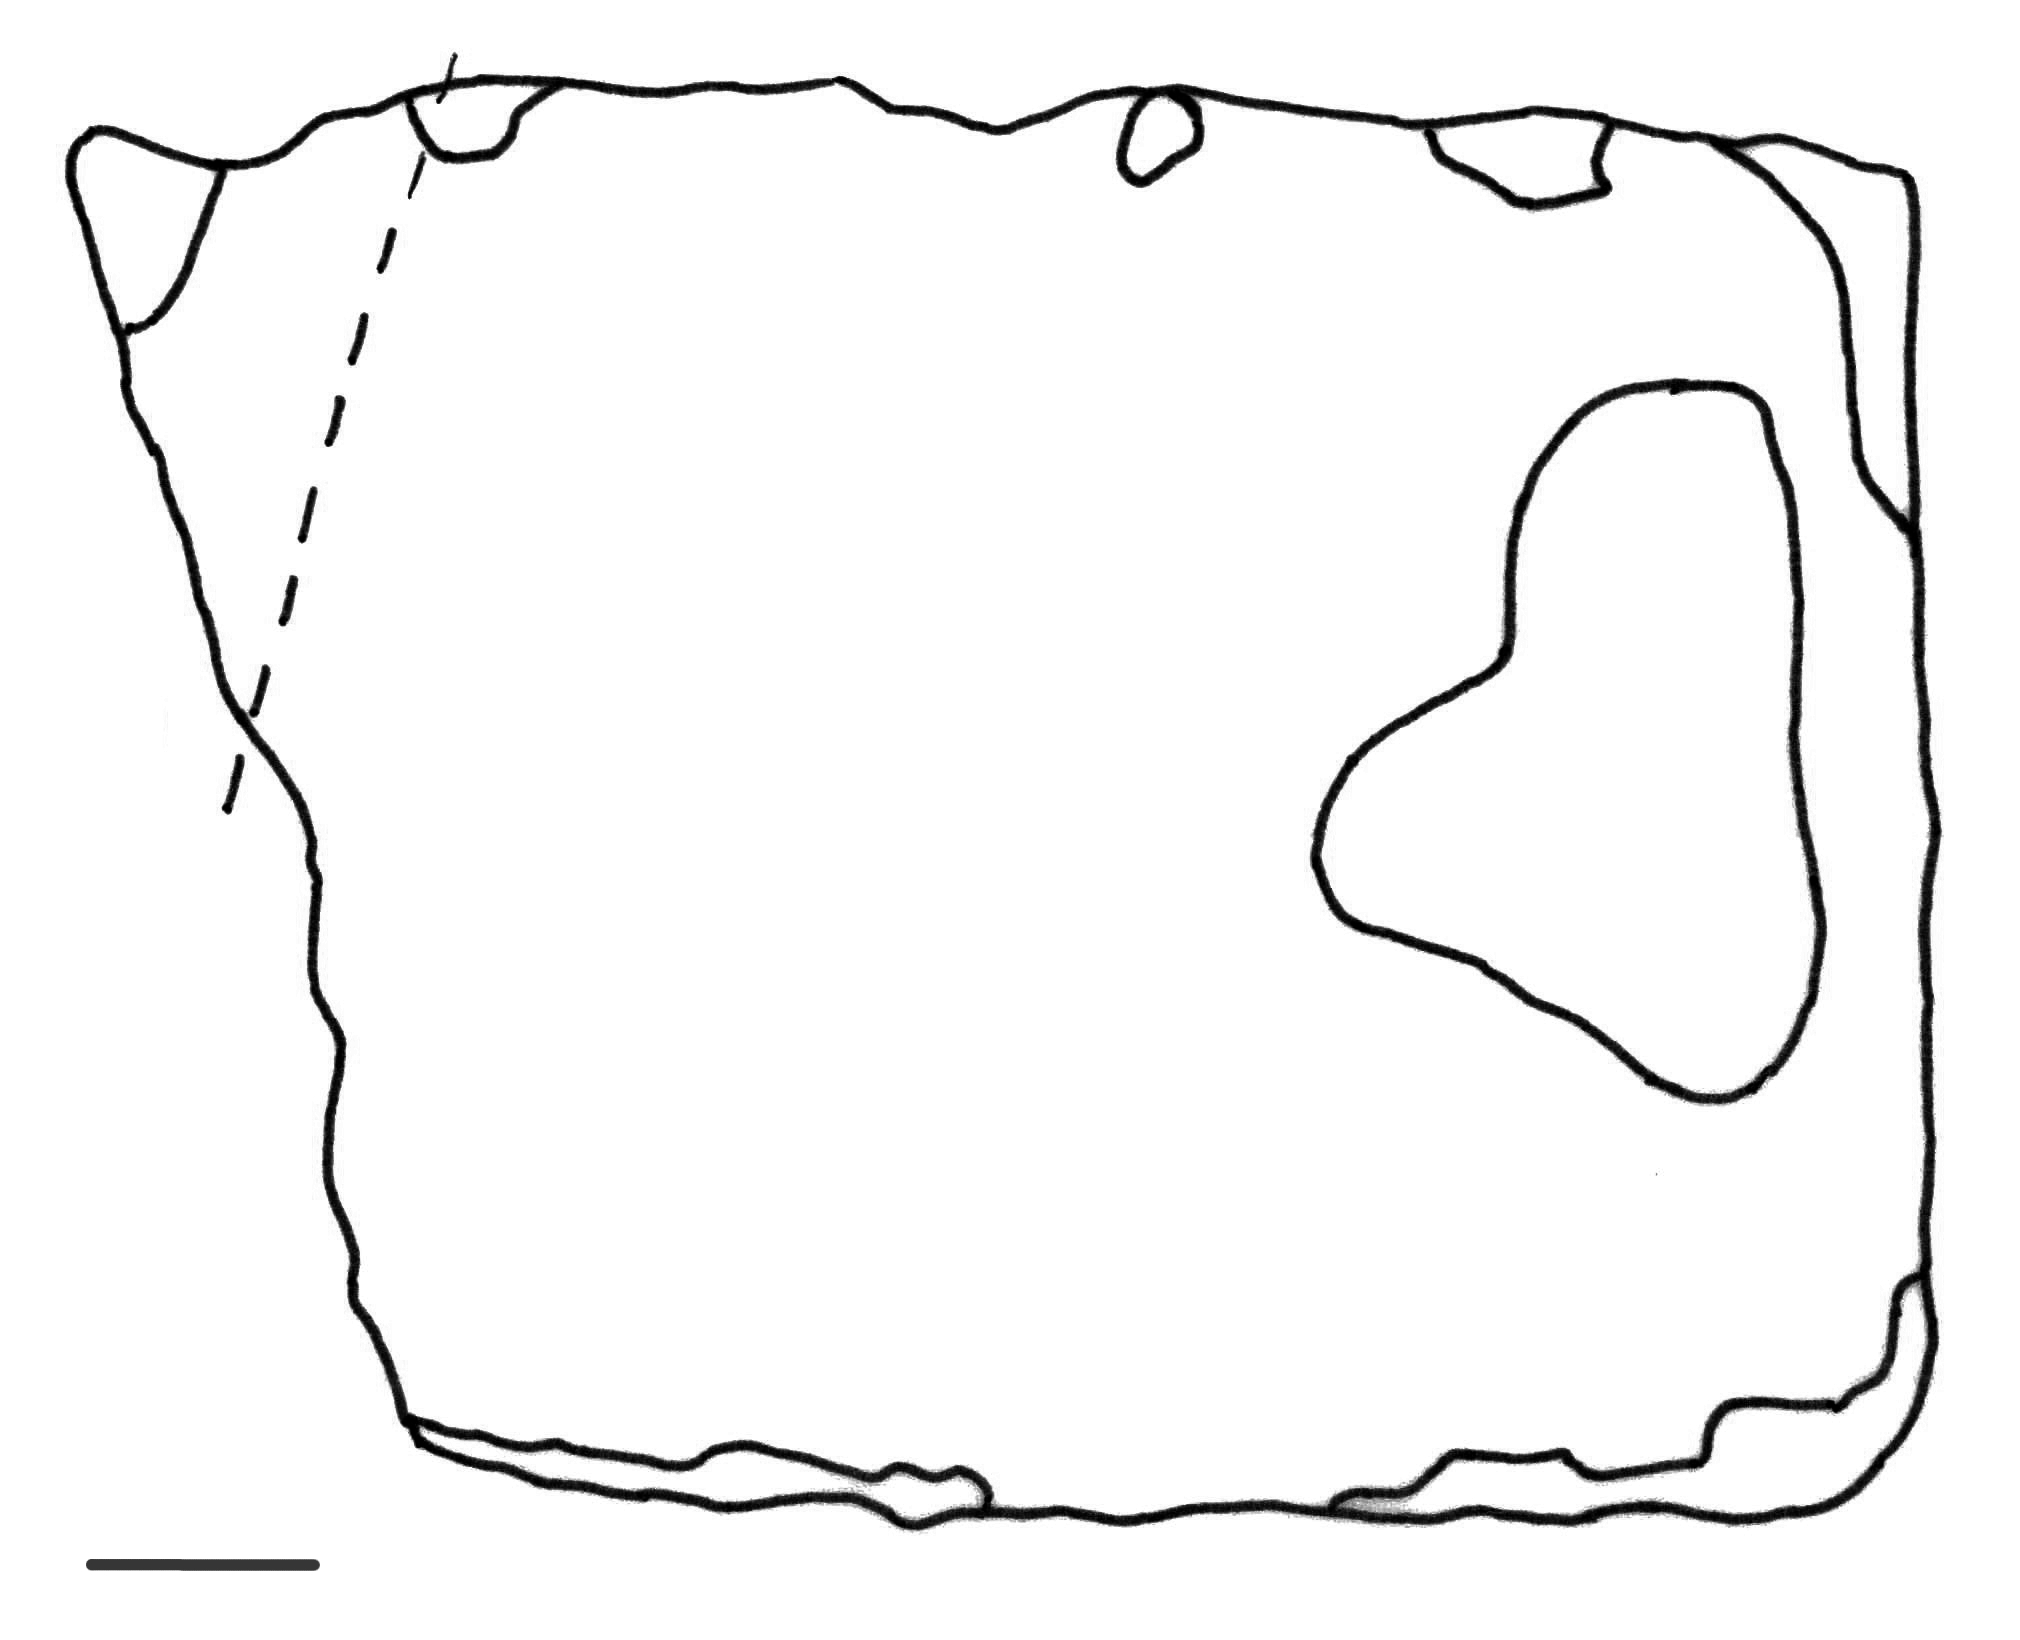
\includegraphics[scale=0.17]{PaM_BDX6529_dessus}
    \subcaption{Vue de dessus \label{dessin:6529_dessus}}

    \bigskip
    \bigskip

    % Dessin de l'échantillon : Coupe
    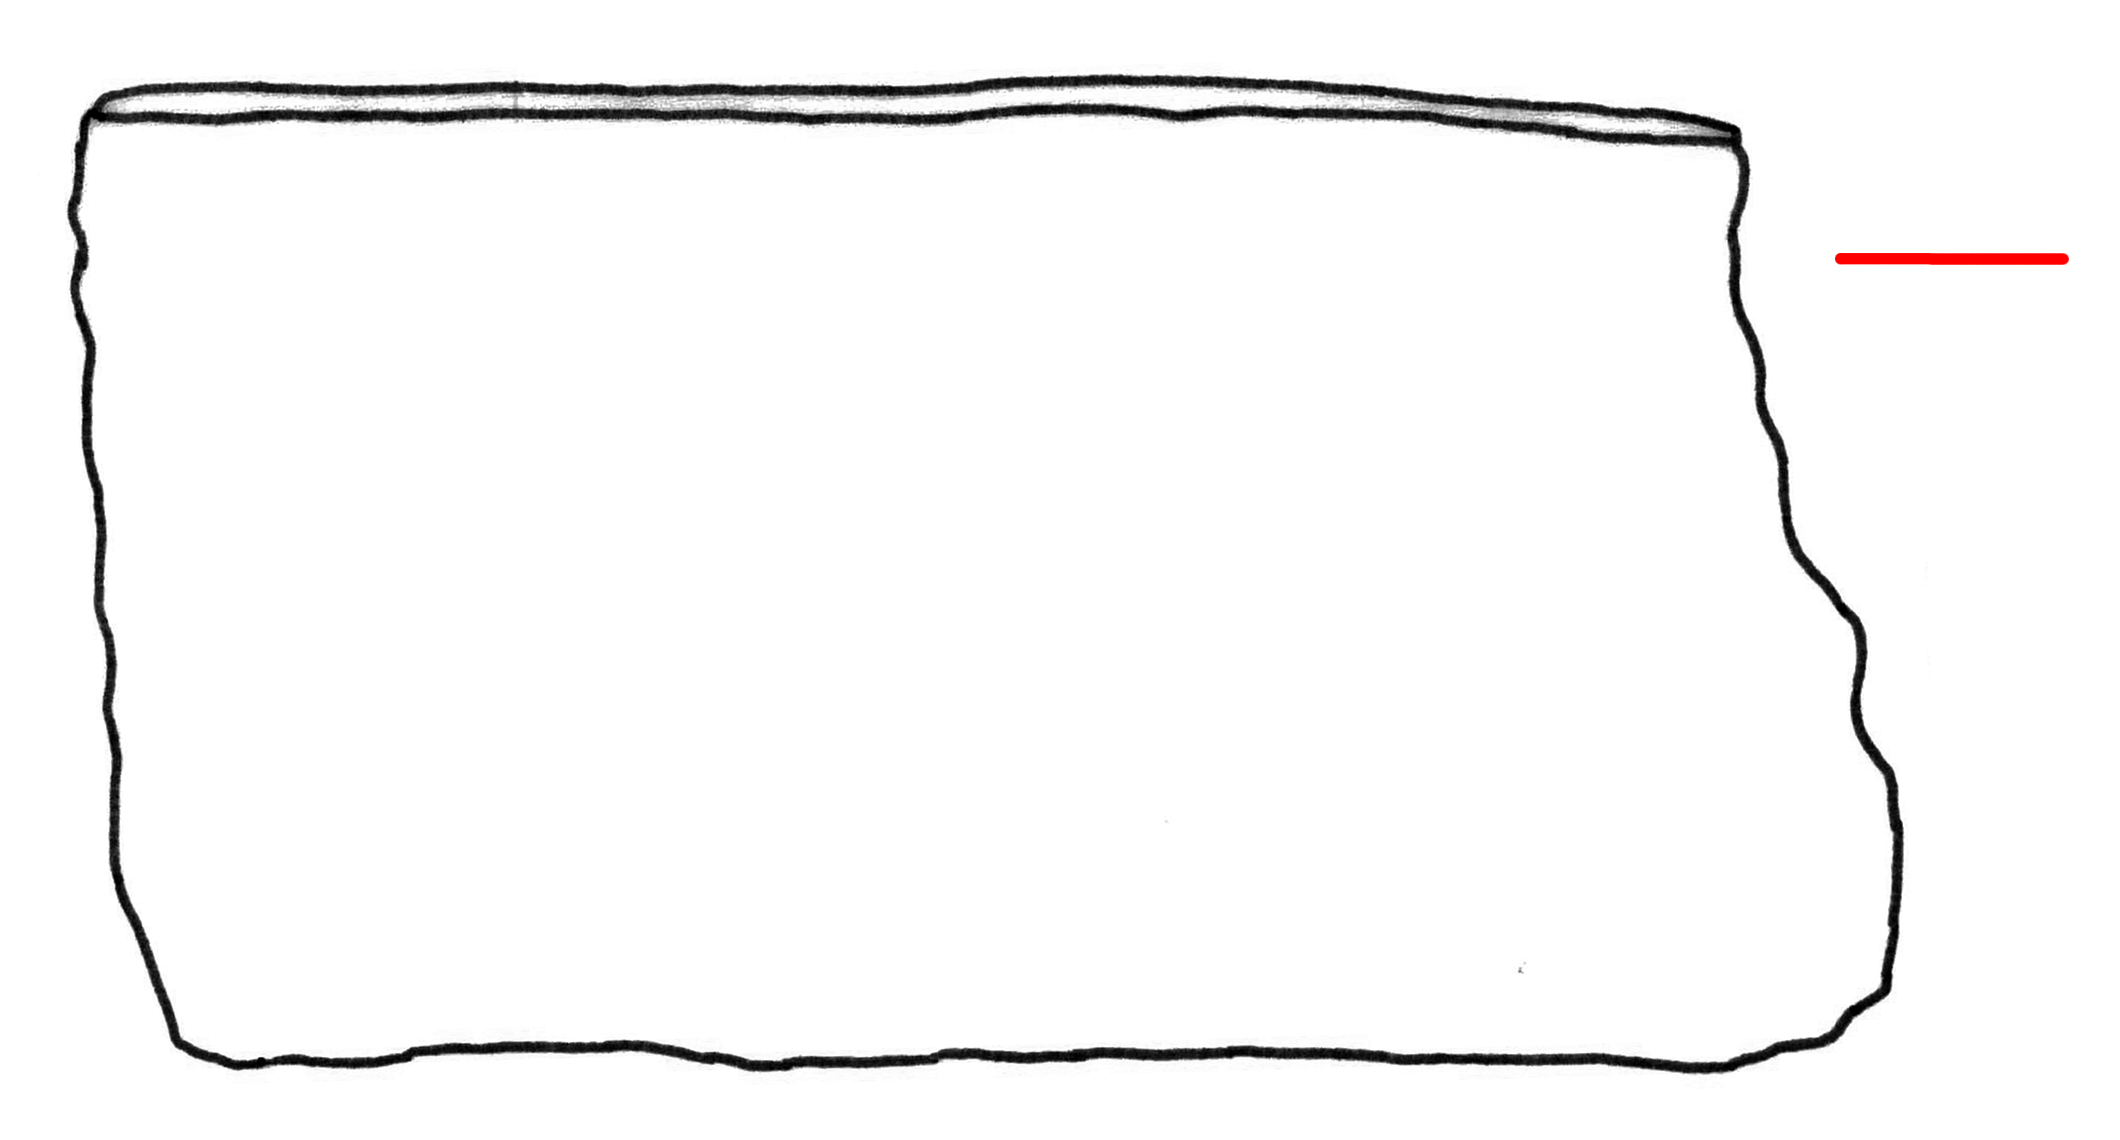
\includegraphics[scale=0.17]{PaM_BDX6529_coupe}
    \subcaption{Vue en coupe \label{dessin:6529_coupe}}
  \end{minipage}%
  \qquad%
  \begin{minipage}[t]{6.2cm}
    \centerfloat
    \vspace*{0pt}
    % Dessin de l'échantillon : Lame
    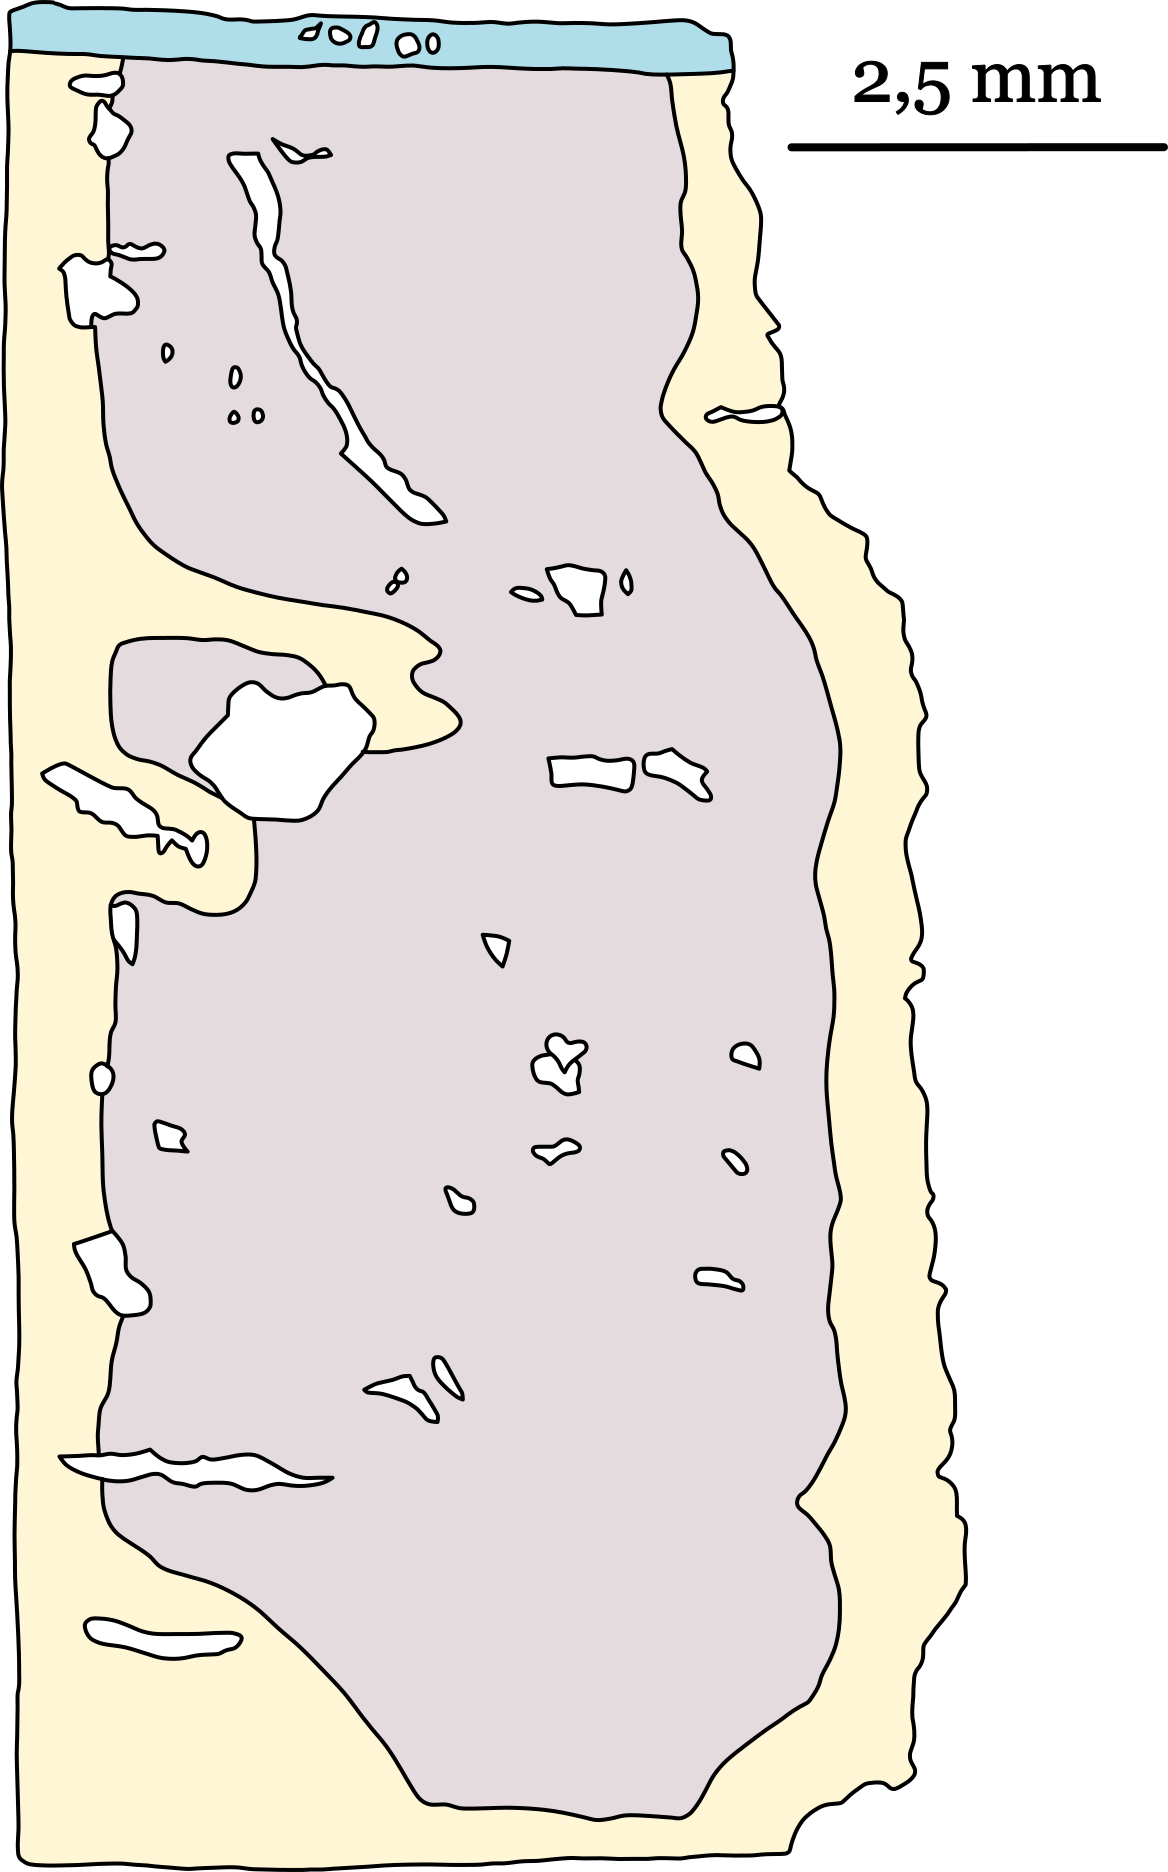
\includegraphics[scale=0.17]{PaM_BDX6529_lame}
    \subcaption{Lame étudiée \label{dessin:6529_lame}}

    \bigskip
    \bigskip
    \bigskip

    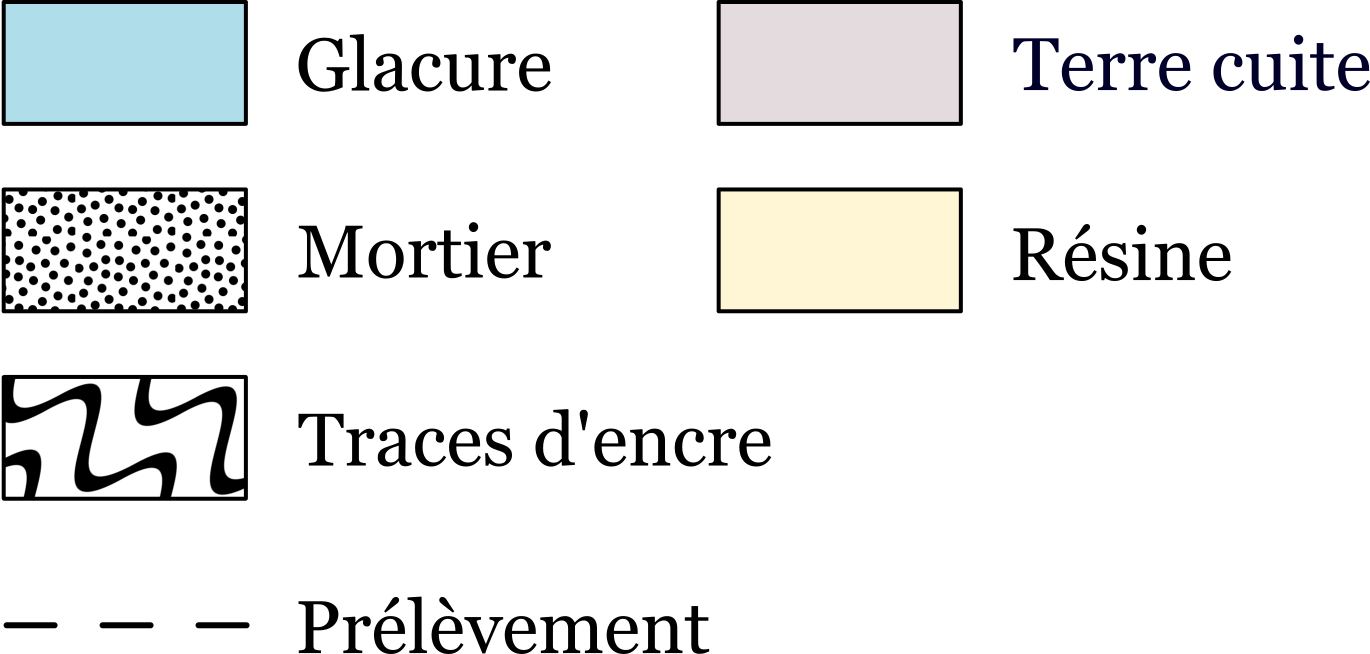
\includegraphics[scale=0.17]{PaM_BDX6529_legende}
  \end{minipage}
  \caption[\bdx{6529}]{\legendeB.}
  \label{dessin:6529}
\end{figure}

L'observation de la surface de la glaçure (\fref{surf:6529}) montre 
qu'elle est opaque et contient des bulles. Elle présente également 
une forte usure mécanique pouvant s'expliquer par le fait que 
l'échantillon provient d'un pavement de sol.

Le support de terre cuite est de couleur rougeâtre, de granulométrie 
fine, et contient quelques porosités de grande taille ainsi que des 
inclusions rouges et blanches.

\begin{figure}[htb]
  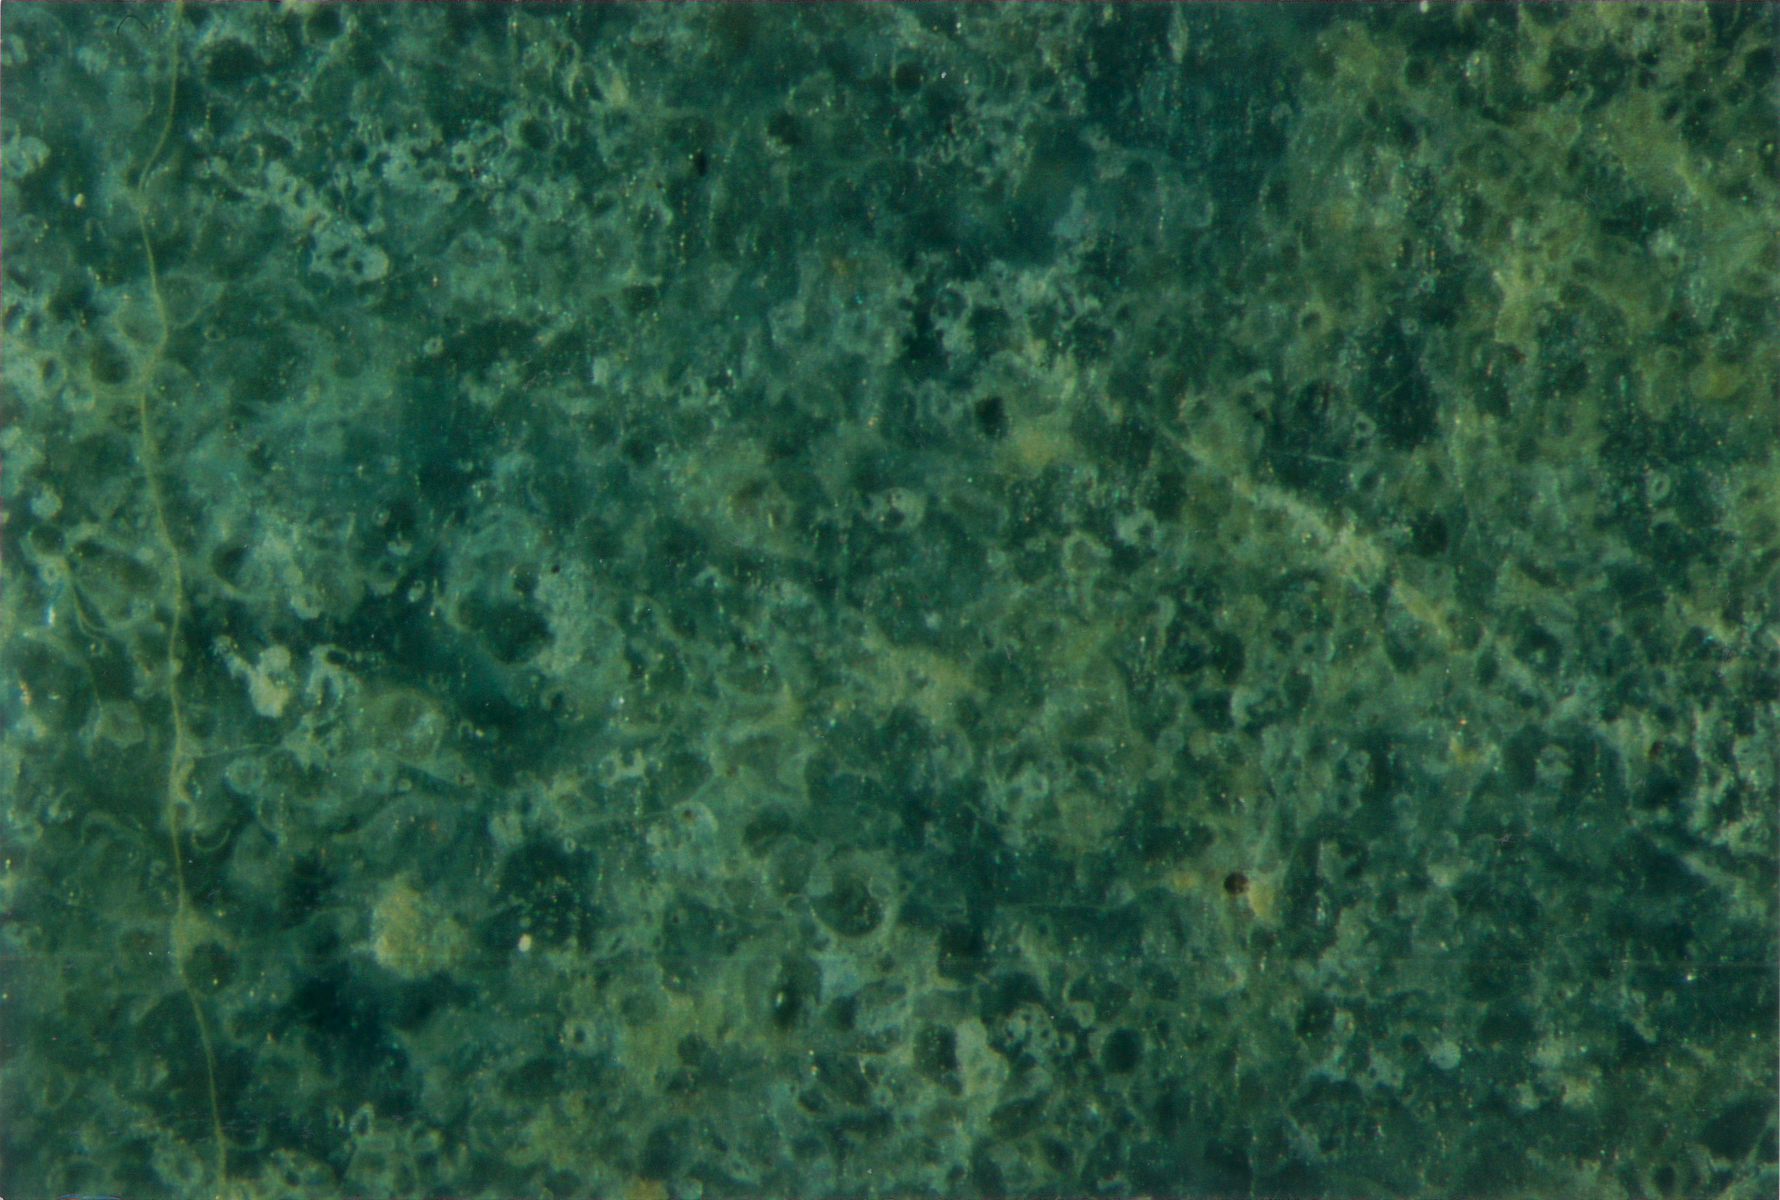
\includegraphics[width=\textwidth]{PaM_BDX6529_Surf}
  \caption[\bdx{6529}\ -- État de surface de la glaçure]
          {\legendeB.
           État de surface de la glaçure 
           (Gr=\num{30}, \zone{\sim4.3x3.2}{\mm}). 
           Elle contient des bulles et présente une forte usure 
           de surface.}
  \label{surf:6529}
\end{figure}


\section{Étude de la couleur}
%----------------------------------------------------------------------

\subsection{Identification des ions chromogènes}
%~~~~~~~~~~~~~~~~~~~~~~~~~~~~~~~~~~~~~~~~~~~~~~~~~~~~~~~~~~~~~~~~~~~~~~
Le spectre d'\AO en mode réflexion diffuse de la glaçure bleu vert 
(\fref{spectre:6529}) laisse apparaître trois bandes d'absorption à 
\SIlist{525;600;660}{\nm}, caractéristiques du \ch{Co^2+} 
\autocite{Lajarte_1979}.

\begin{figure}[htb]
  \begin{plotspectre}
    \addplot [thick, PowderBlue!75!black] 
       table [x=lambda, y=6529gla] {\gladata} ;
    \addlegendentry{glaçure bleue}
    \addplot [thick, PowderBlue!50!black] 
       table [x=lambda, y=6529glaSPMO] {\gladata} ;
    \addlegendentry{glaçure bleue, SPMO}
    \addplot [thick, FireBrick] 
       table [x=lambda, y=6529tc] {\tcdata} ;
    \addlegendentry{terre cuite}

    \begin{scope}[<-, >=stealth, shorten <=5pt, thin]
      \node (Co) at (595.00, 0.80) {\ch{Co^2+}} ;
      \draw (525.00, 0.56) |- (Co.south) ;
      \draw (600.00, 0.61) |- (Co.south) ;
      \draw (660.00, 0.59) |- (Co.south) ;
    \end{scope}
  \end{plotspectre}
  \caption[\bdx{6529}\ -- Spectres d'\AO en mode réflexion diffuse 
           de la glaçure et de la terre cuite]
          {\legendeB.
           Spectres d'\AO en mode réflexion diffuse de la glaçure et 
           de la terre cuite. La coloration de la glaçure est due au 
           \ch{Co^2+} mis en évidence par les trois bandes 
           d'absorption à \SIlist{525;600;660}{\nm}.}
  \label{spectre:6529}
\end{figure}

\subsection{Mesure physique de la couleur}
%~~~~~~~~~~~~~~~~~~~~~~~~~~~~~~~~~~~~~~~~~~~~~~~~~~~~~~~~~~~~~~~~~~~~~~
À partir du spectre d'\AO, ont été calculées les coordonnées 
chromatiques correspondant aux espaces \Yxy et \Lab 
(\tref{saotab:6529}). La longueur d'onde dominante associée 
au rayonnement correspond au domaine du vert jaunâtre 
\autocite{Kelly_1976}. Ce résultat, en contradiction avec 
l'observation visuelle, peut s'expliquer par la forte usure de la 
glaçure. En effet, elle laisse par endroit apparaître le support 
céramique rougeâtre sous-jacent, ce qui altère la perception de la 
couleur de la glaçure.

Nous avons donc utilisé un montage spectrophotomètre/microscope 
optique (Gr=40) permettent de focaliser le faisceau pour analyser 
une zone saine de la glaçure. Le spectre obtenu présente, lui aussi, 
les trois bandes d'absorption caractéristiques du \ch{Co^2+}. 
Les résultats de \CHRO sont consignés dans le \tref{saotab:6529} et 
la \fref{colorfig:6529} en donne les représentations graphiques. 
La longueur d'onde dominante est cette fois de \SI{482.54}{\nm}, 
elle correspond au domaine du bleu verdâtre \autocite{Kelly_1976}. 
La pureté d'excitation \SI{3.71}{\percent} est celle d'une couleur très 
peu saturée, la réflectance \CIEY (\num{27.839}) indique une couleur 
assez foncée.

\begin{table}[hbt]
  \caption[\bdx{6529}\ -- Coordonnées chromatiques et longueur d'onde 
           dominante]
          {\legendeB.
           Coordonnées chromatiques dans les systèmes \Yxy et \Lab 
           et longueur d'onde dominante (illuminant D65, \ang{2},
           \SIrange{400}{700}{\nm}). (\up{\dag}\,\cite{Kelly_1976})}
  \label{saotab:6529}
  \begin{chrotab}[Appareillage]
      \chrolgna{Spectro\-photo\-mètre}{551.45}{3.81}
               {27.953}{0.313}{0.343}
               {59.847}{-4.345}{3.382} &
      \chrolgnb{vert jaunâtre foncé}{Vert-Jaune}{530}{560}{}
    \tabularnewline
      \chrolgna{Spectro\-photo\-mètre + microscope optique}
               {482.54}{3.71}
               {27.839}{0.304}{0.323}
               {59.743}{-1.006}{-2.601} &
      \chrolgnb{bleu verdâtre foncé}{Bleu-verdâtre}{482}{487}{}
               % {\footnotemark{}}
    \tabularnewline
  \end{chrotab}
\end{table}
% \footnotetext{\autocite{Kelly_1976}}

\begin{figure}[htb]
  \newcommand{\samplename}{6529gla}
  \newcommand{\samplecolor}{PowderBlue}
  \begin{minipage}[t]{0.37\paperwidth}
    \begin{plotYxy}
      \plotYxyPaV ;
      \plotYxyIlluminant ;
      \plotYxySample{\samplename}{\samplecolor} ;
      \plotYxyLigne{\samplename} ;
      \plotYxyAnnot{\samplename}{north west} ;
    \end{plotYxy}
    \subcaption[Espace \trichro \Yxy]
               {Espace \trichro \Yxy. La longueur d'onde 
                dominante de la glaçure est de \SI{482.54}{\nm} et 
                correspond au domaine du bleu vert. La couleur est 
                très peu saturée : son point représentatif est très 
                proche de l'illuminant standard.}
  \end{minipage}%
  \qquad%
  \begin{minipage}[t]{0.37\paperwidth}
    \begin{plotLab}
      \plotLabSample{\samplename}{\samplecolor} ;
    \end{plotLab}
    \subcaption[Espace \trichro \Lab]
               {Espace \trichro \Lab. Le point représentatif de 
                la couleur de la glaçure est dans le quart vert-bleu.}
  \end{minipage}%
  \caption[\bdx{6529}\ -- Analyse chromamétrique de la glaçure]
          {\legendeB. Analyse chromamétrique de la glaçure.}
  \label{colorfig:6529}
\end{figure}


\section{Étude de la texture de la glaçure et de la terre cuite}
%----------------------------------------------------------------------

\subsection{Observation en lumière naturelle}
%~~~~~~~~~~~~~~~~~~~~~~~~~~~~~~~~~~~~~~~~~~~~~~~~~~~~~~~~~~~~~~~~~~~~~~
\begin{figure}[htb]
  \begin{minipage}[t]{0.48\textwidth}
    \centerfloat
    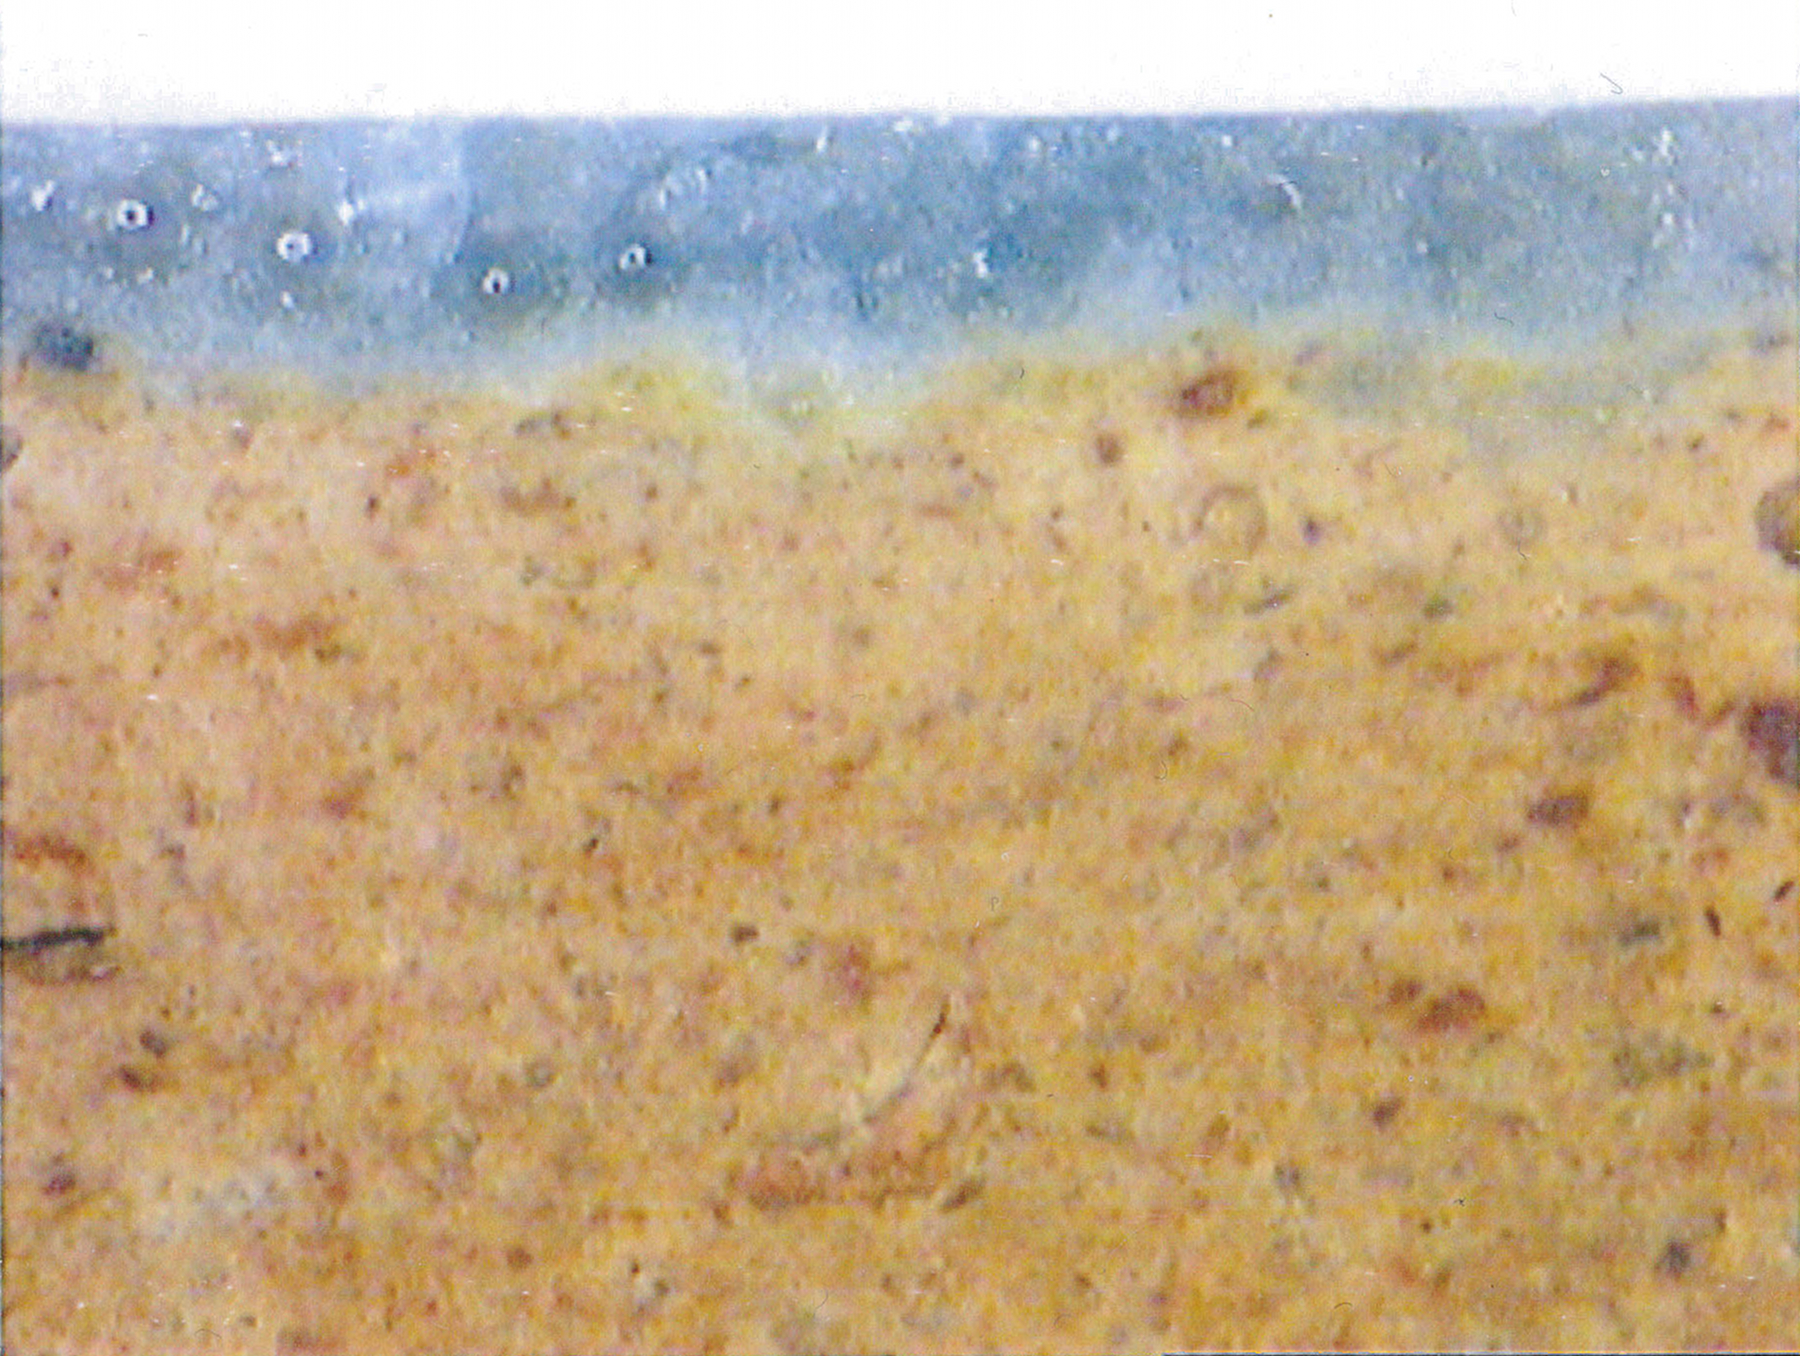
\includegraphics[width=\textwidth]{PaM_BDX6529_LN}%
    \subcaption{Lumière naturelle \label{texture:6529_LN}}
  \end{minipage}%
  \hfill%
  \begin{minipage}[t]{0.48\textwidth}
    \centerfloat
    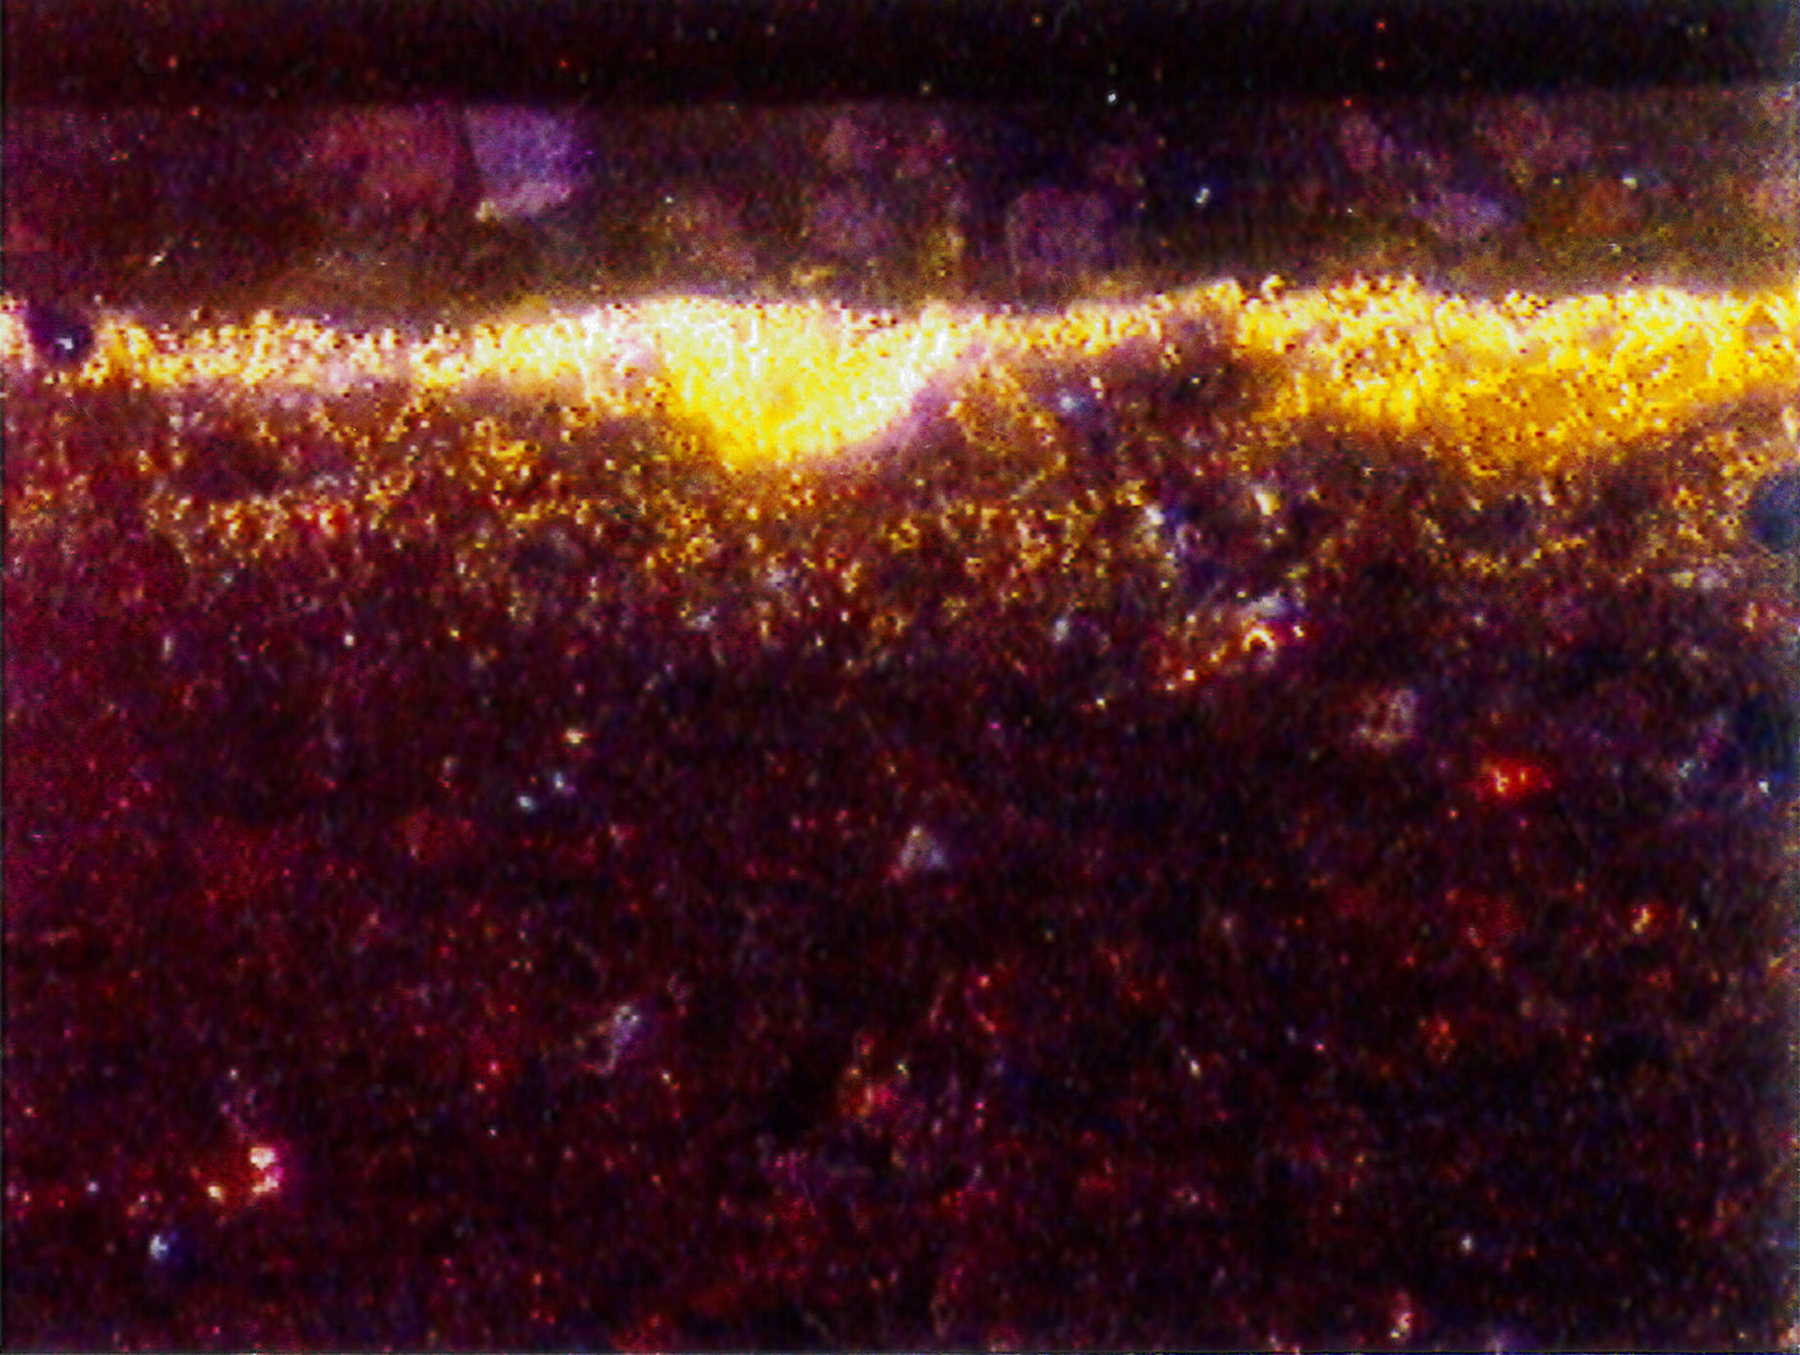
\includegraphics[width=\textwidth]{PaM_BDX6529_CL}%
    \subcaption{\CL \label{texture:6529_CL}}
  \end{minipage}
  \caption[\bdx{6529}\ -- Observation de la texture en section]
          {\legendeB.
           Observation de la texture en section 
           sur une surface de \SI{2.6x1.9}{\mm}.}
  \label{texture:6529}
\end{figure}

L'examen en section en lumière naturelle de l'ensemble terre 
cuite-glaçure (\fref{texture:6529_LN}), montre que la glaçure est 
colorée dans la masse et qu'elle adhère bien au support de terre cuite.

Cette dernière contient peu d'inclusions, blanches et rouges.

\subsection{Observation en \CL}
%~~~~~~~~~~~~~~~~~~~~~~~~~~~~~~~~~~~~~~~~~~~~~~~~~~~~~~~~~~~~~~~~~~~~~~
On peut distinguer dans l'ensemble de la glaçure 
(\fref{texture:6529_CL}), des cristaux présentant une 
luminescence mauve.

La terre cuite luminesce elle aussi en mauve. Elle contient quelques 
inclusions qui luminescent en rouge et en bleu.

Sur toute la largeur de la lame étudiée, on note la présence d'un 
large liseré luminescent en jaune à l'interface glaçure-terre cuite.


\subsection{Observation en \MEB[ie]}
%~~~~~~~~~~~~~~~~~~~~~~~~~~~~~~~~~~~~~~~~~~~~~~~~~~~~~~~~~~~~~~~~~~~~~~
La glaçure a une épaisseur moyenne de \SI{300}{\um}. Elle contient 
des bulles et de nombreux cristaux non fondus, dont la dimension peut 
aller jusqu'à \SI{100}{\um}. Elle semble avoir pénétré par endroits 
dans la terre cuite (\fref{MEB:6529_img}).

% \begin{figure}[htb]
%   \setlength{\imgwidth}{7cm}
%   \begin{minipage}{.4\textwidth}
%     \centerfloat
%     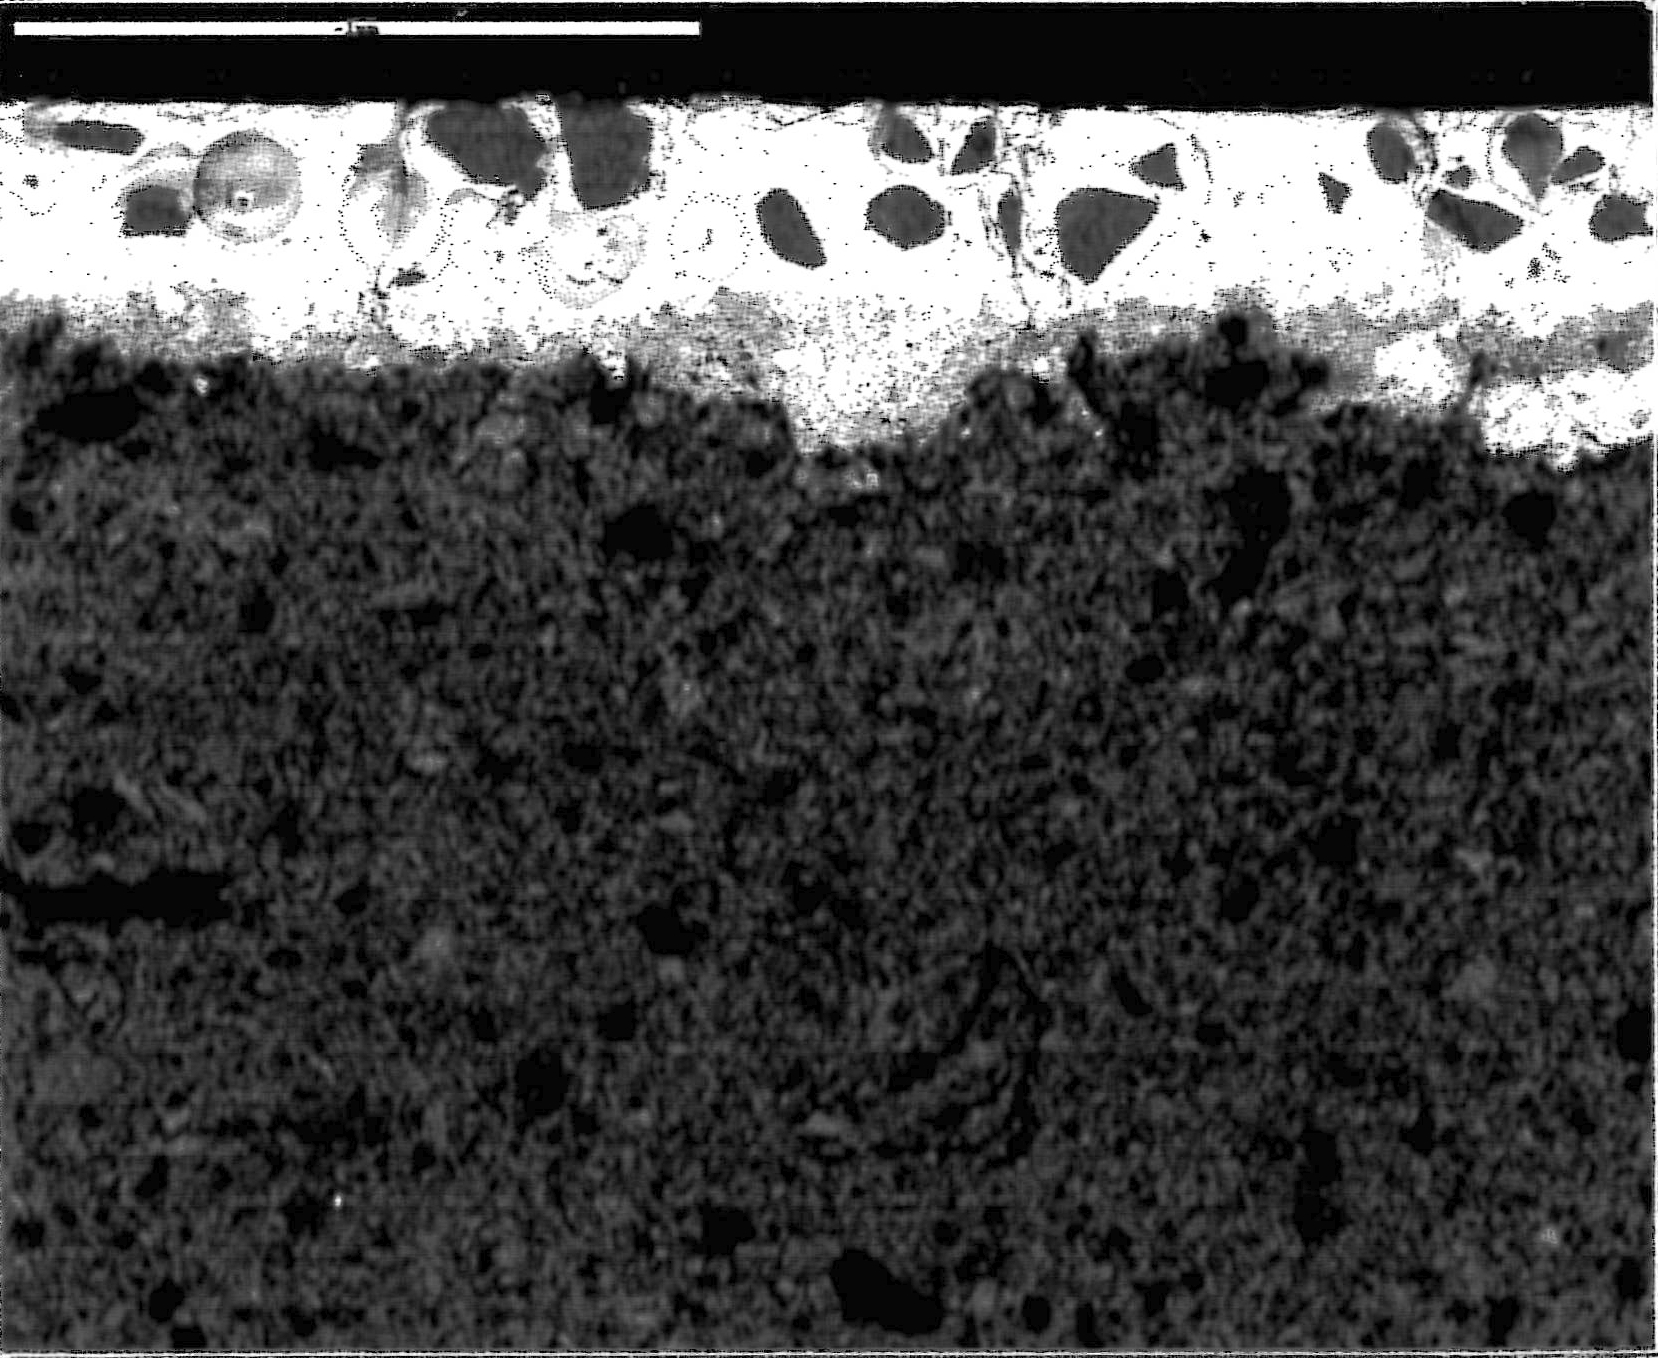
\includegraphics[width=\imgwidth]{PaM_BDX6529_ERD}%
%     \caption[%
%       \bdx{6529}\ -- Observation de la texture au \MEB, 
%       en mode \ERD. Ensemble glaçure-terre cuite%
%     ]{%
%       \legendeB.
%        Observation de la texture au \MEB, en mode \ERD de l'ensemble 
%        glaçure-terre cuite. La barre d'échelle mesure \SI{1}{\mm} 
%        (\zone{2.4x1.9}{\mm}).%
%     }
%     \label{MEB:6529_img}
%   \end{minipage}%
%   \hfill%
%   \begin{minipage}{.4\textwidth}
%     \centerfloat
%     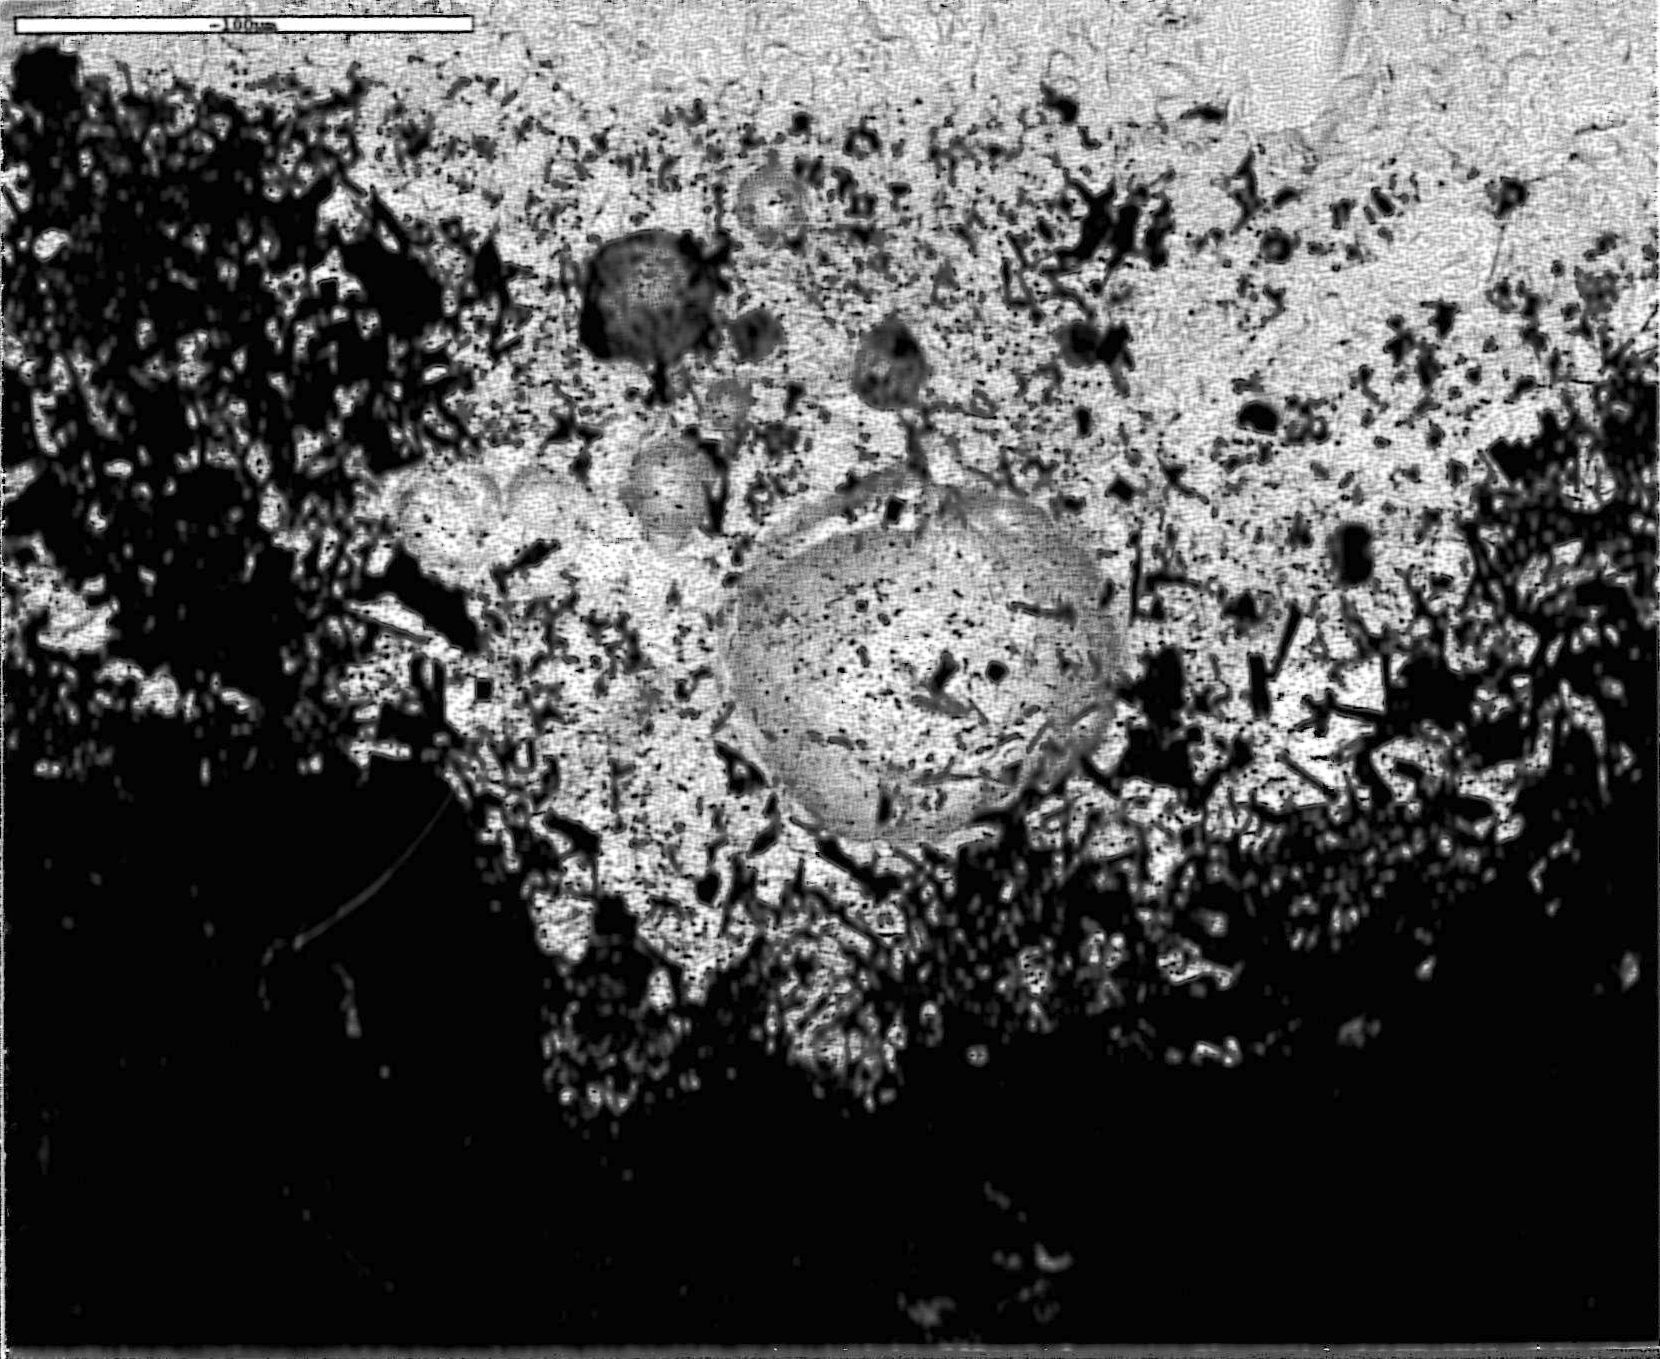
\includegraphics[width=\imgwidth]{PaM_BDX6529_ERD_int}%
%     \caption[%
%       \bdx{6529}\ -- Observation de la texture au \MEB, 
%       en mode \ERD. Interface glaçure-terre cuite%
%     ]{%
%       \legendeB.
%        Observation de la texture au \MEB, en mode \ERD de l'interface 
%        glaçure-terre cuite. La barre d'échelle mesure \SI{100}{\um}
%       ~(\zone{370x300}{\um}).%
%     }
%     \label{MEB:6529_img_int}
%   \end{minipage}%
% \end{figure}

\begin{figure}[htb]
  \setlength{\imgwidth}{7cm}
  % \begin{minipage}[t]{0.48\textwidth}
  \begin{minipage}[t]{\imgwidth}
    \centerfloat
    % 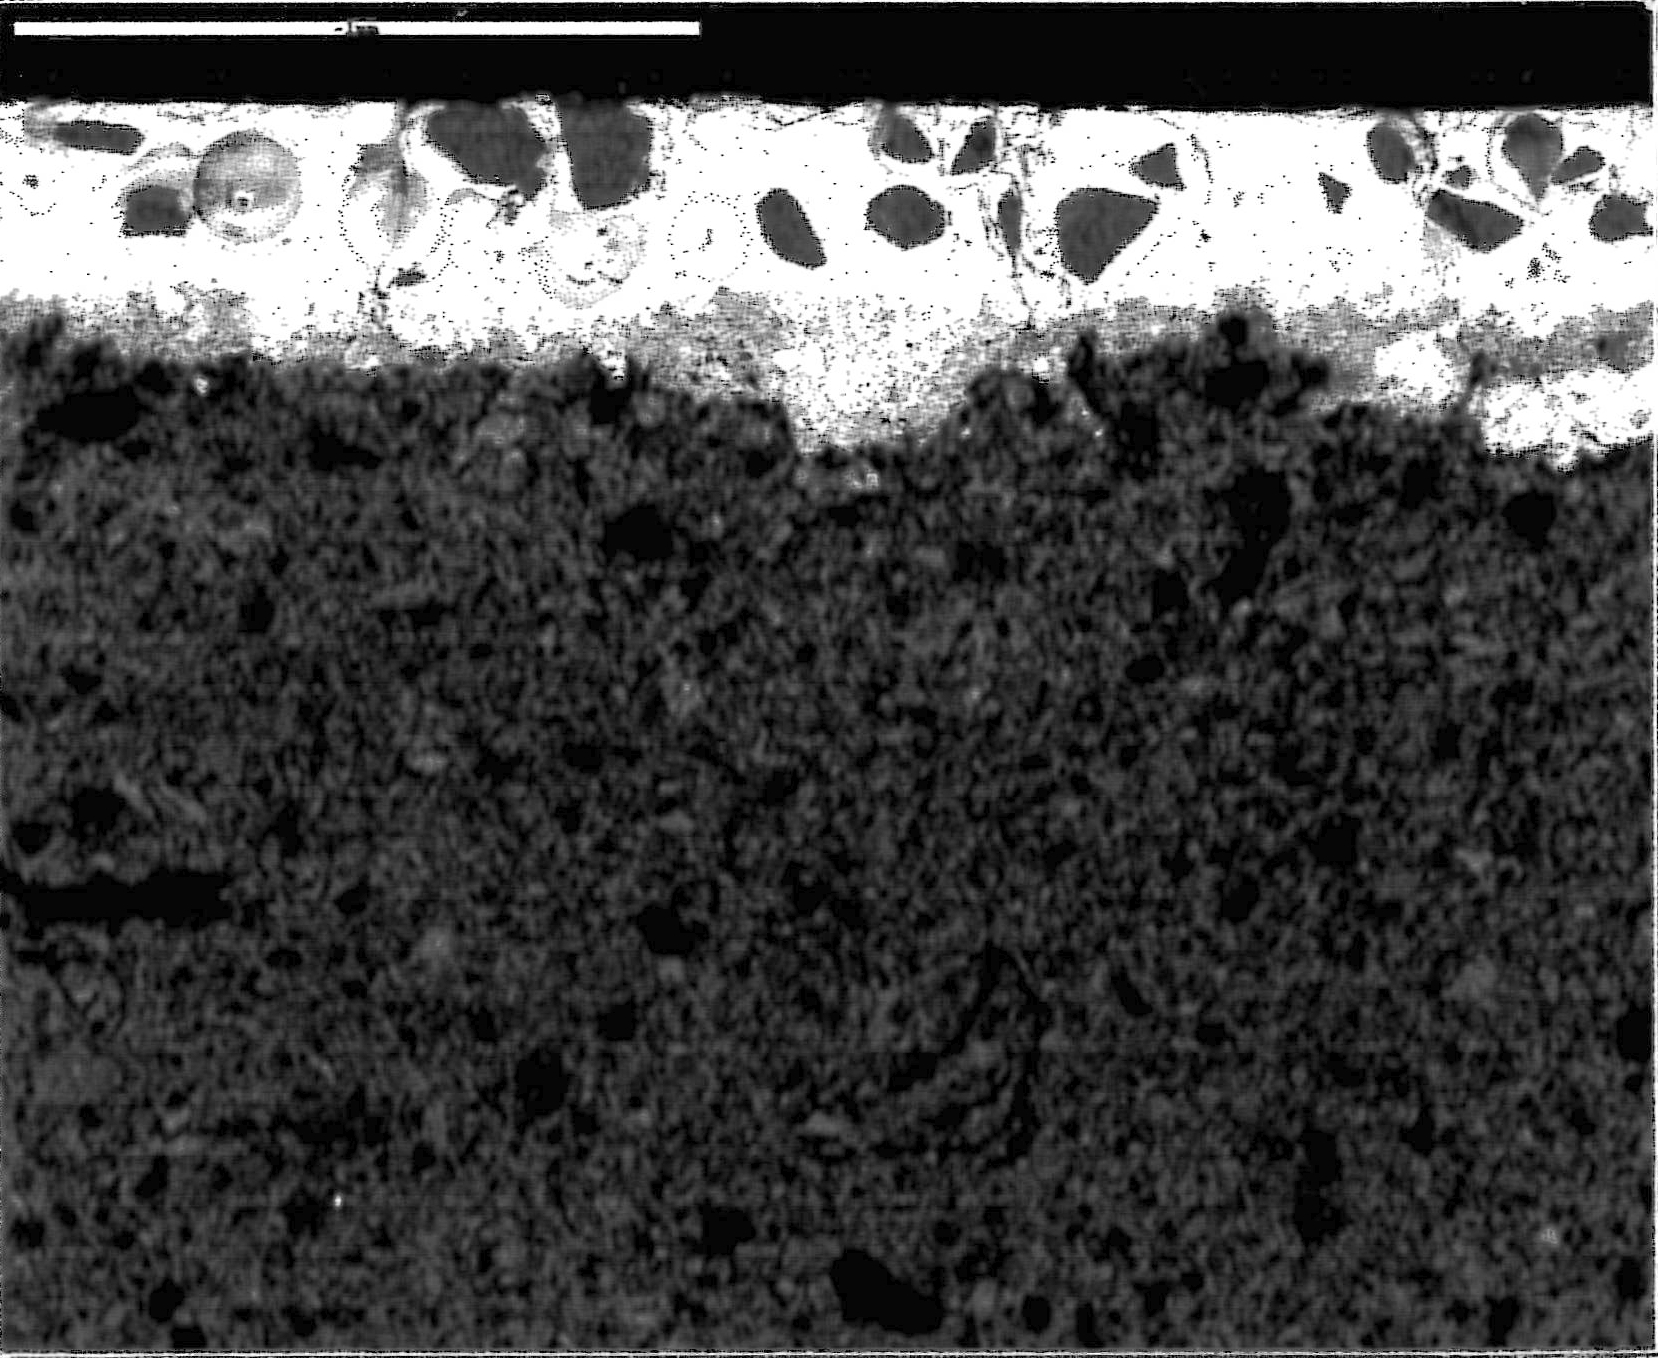
\includegraphics[width=\textwidth]{PaM_BDX6529_ERD}%
    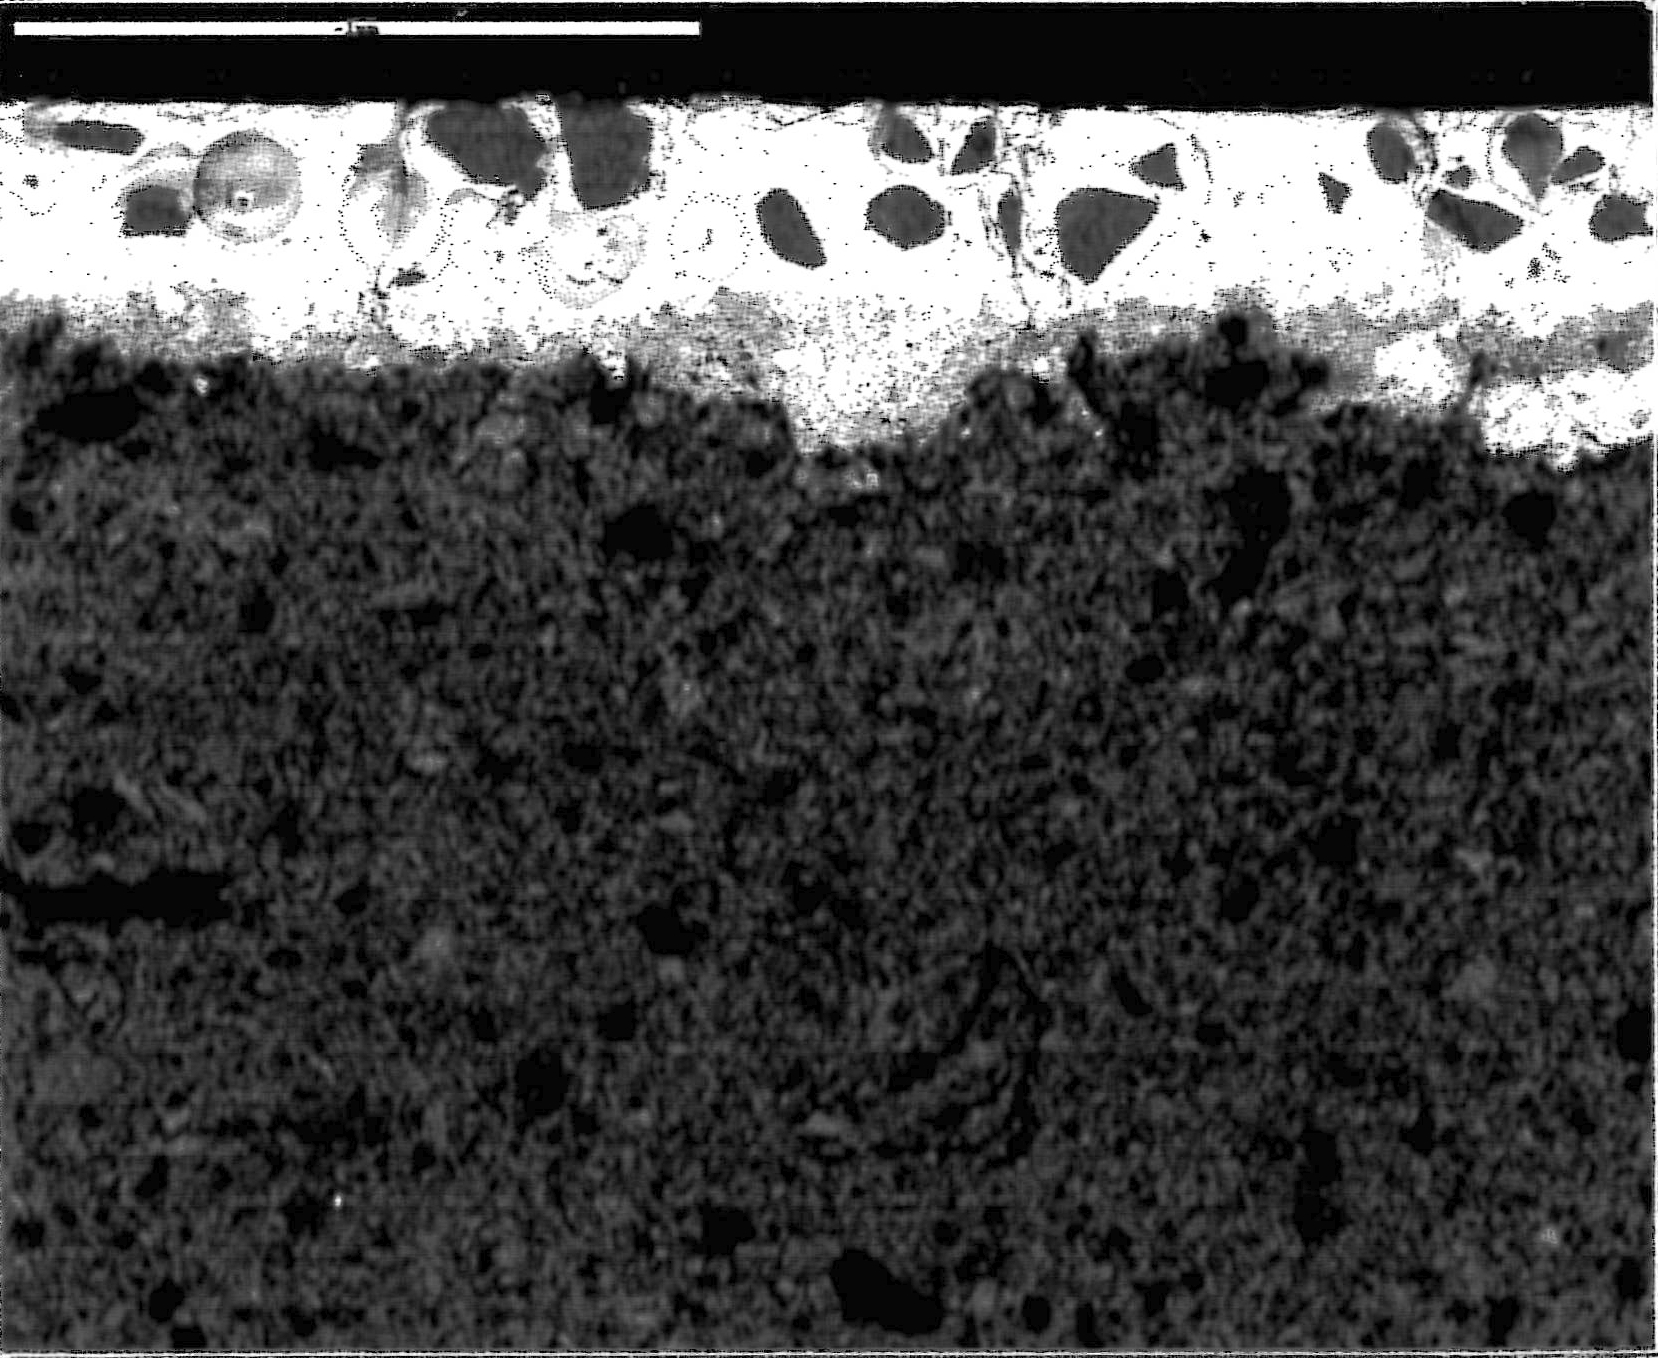
\includegraphics[width=\imgwidth]{PaM_BDX6529_ERD}%
    \subcaption{Interface glaçure-terre cuite. 
                La barre d'échelle mesure \SI{100}{\um}
                (\zone{370x300}{\um}) \label{MEB:6529_img}%
               }
  \end{minipage}%
  \hfill%
  % \begin{minipage}[t]{0.48\textwidth}
  \begin{minipage}[t]{\imgwidth}
    \centerfloat
    % 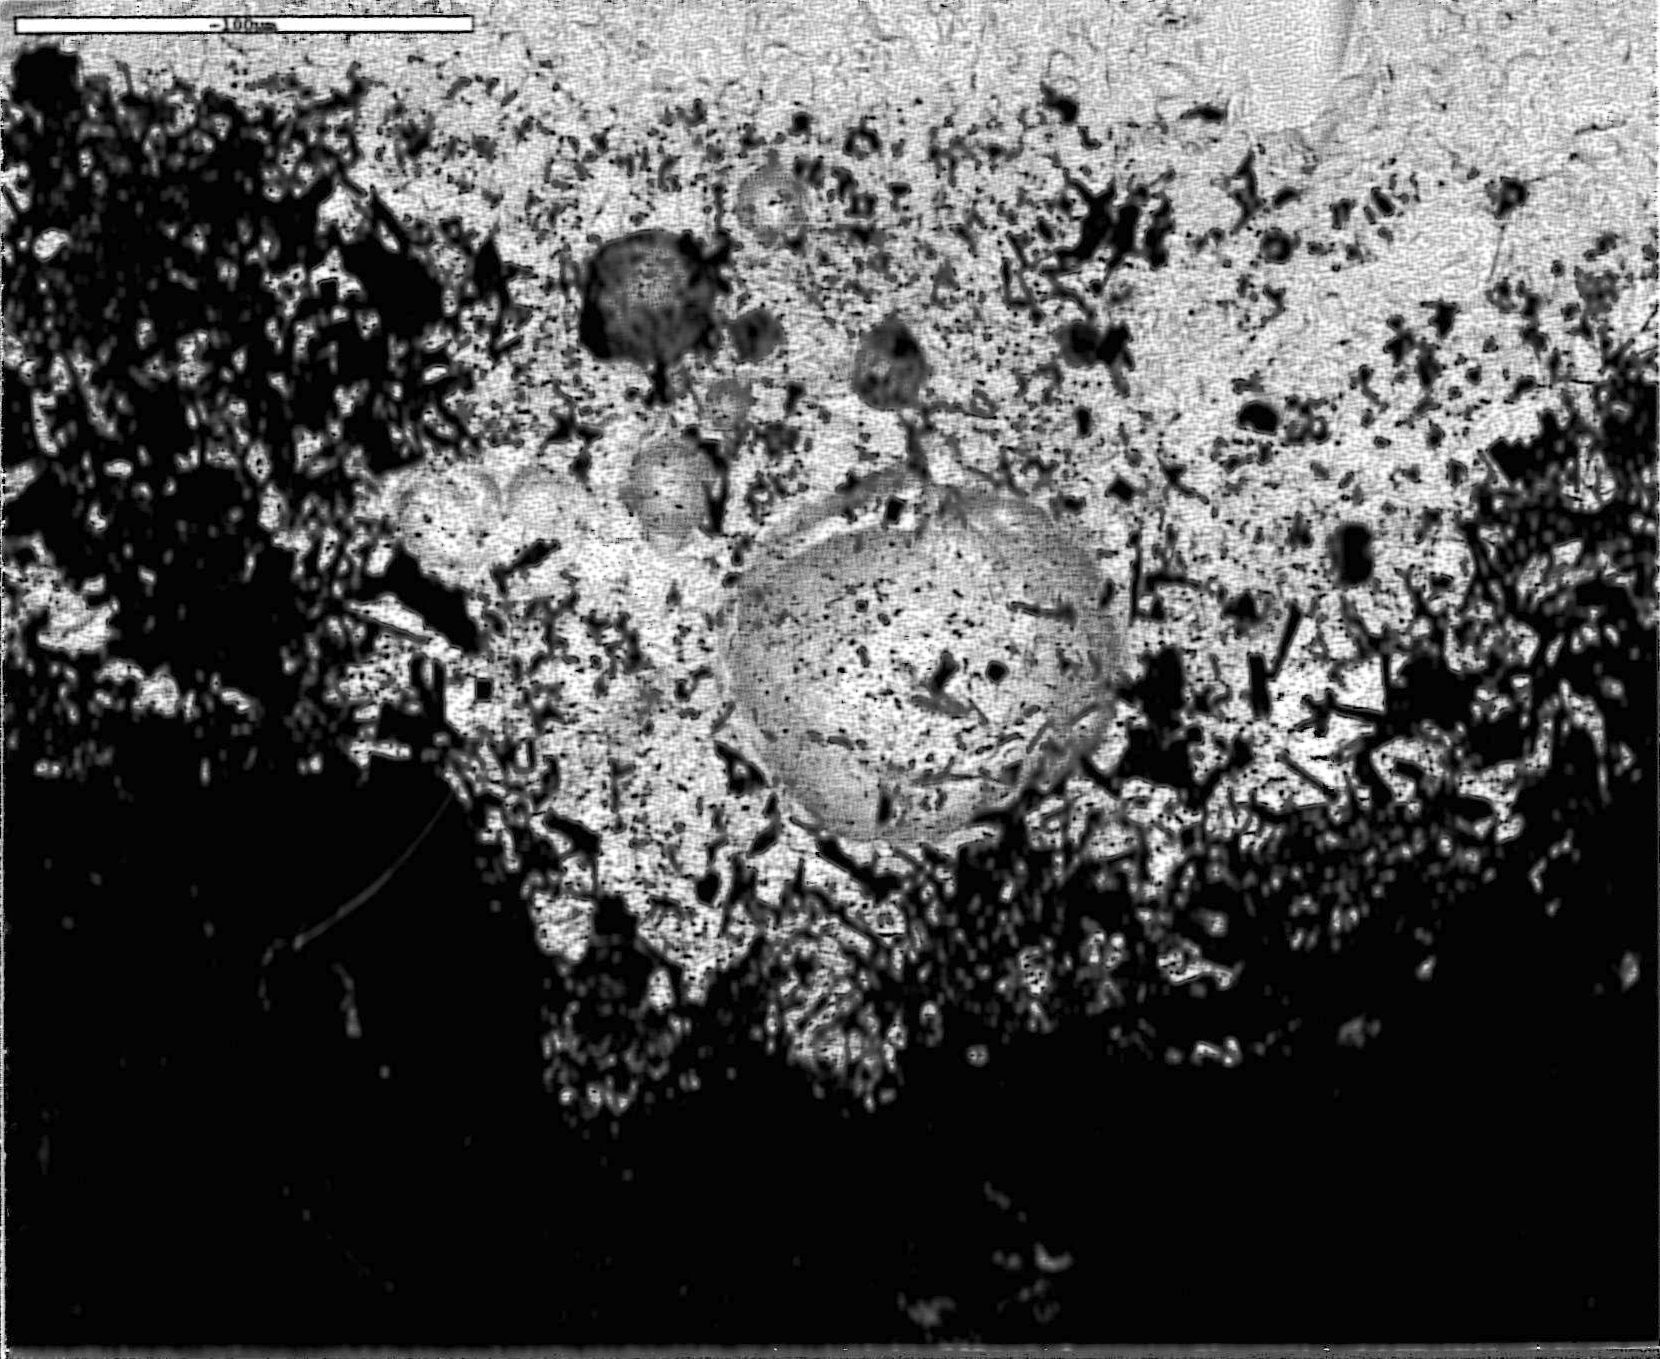
\includegraphics[width=\textwidth]{PaM_BDX6529_ERD_int}%
    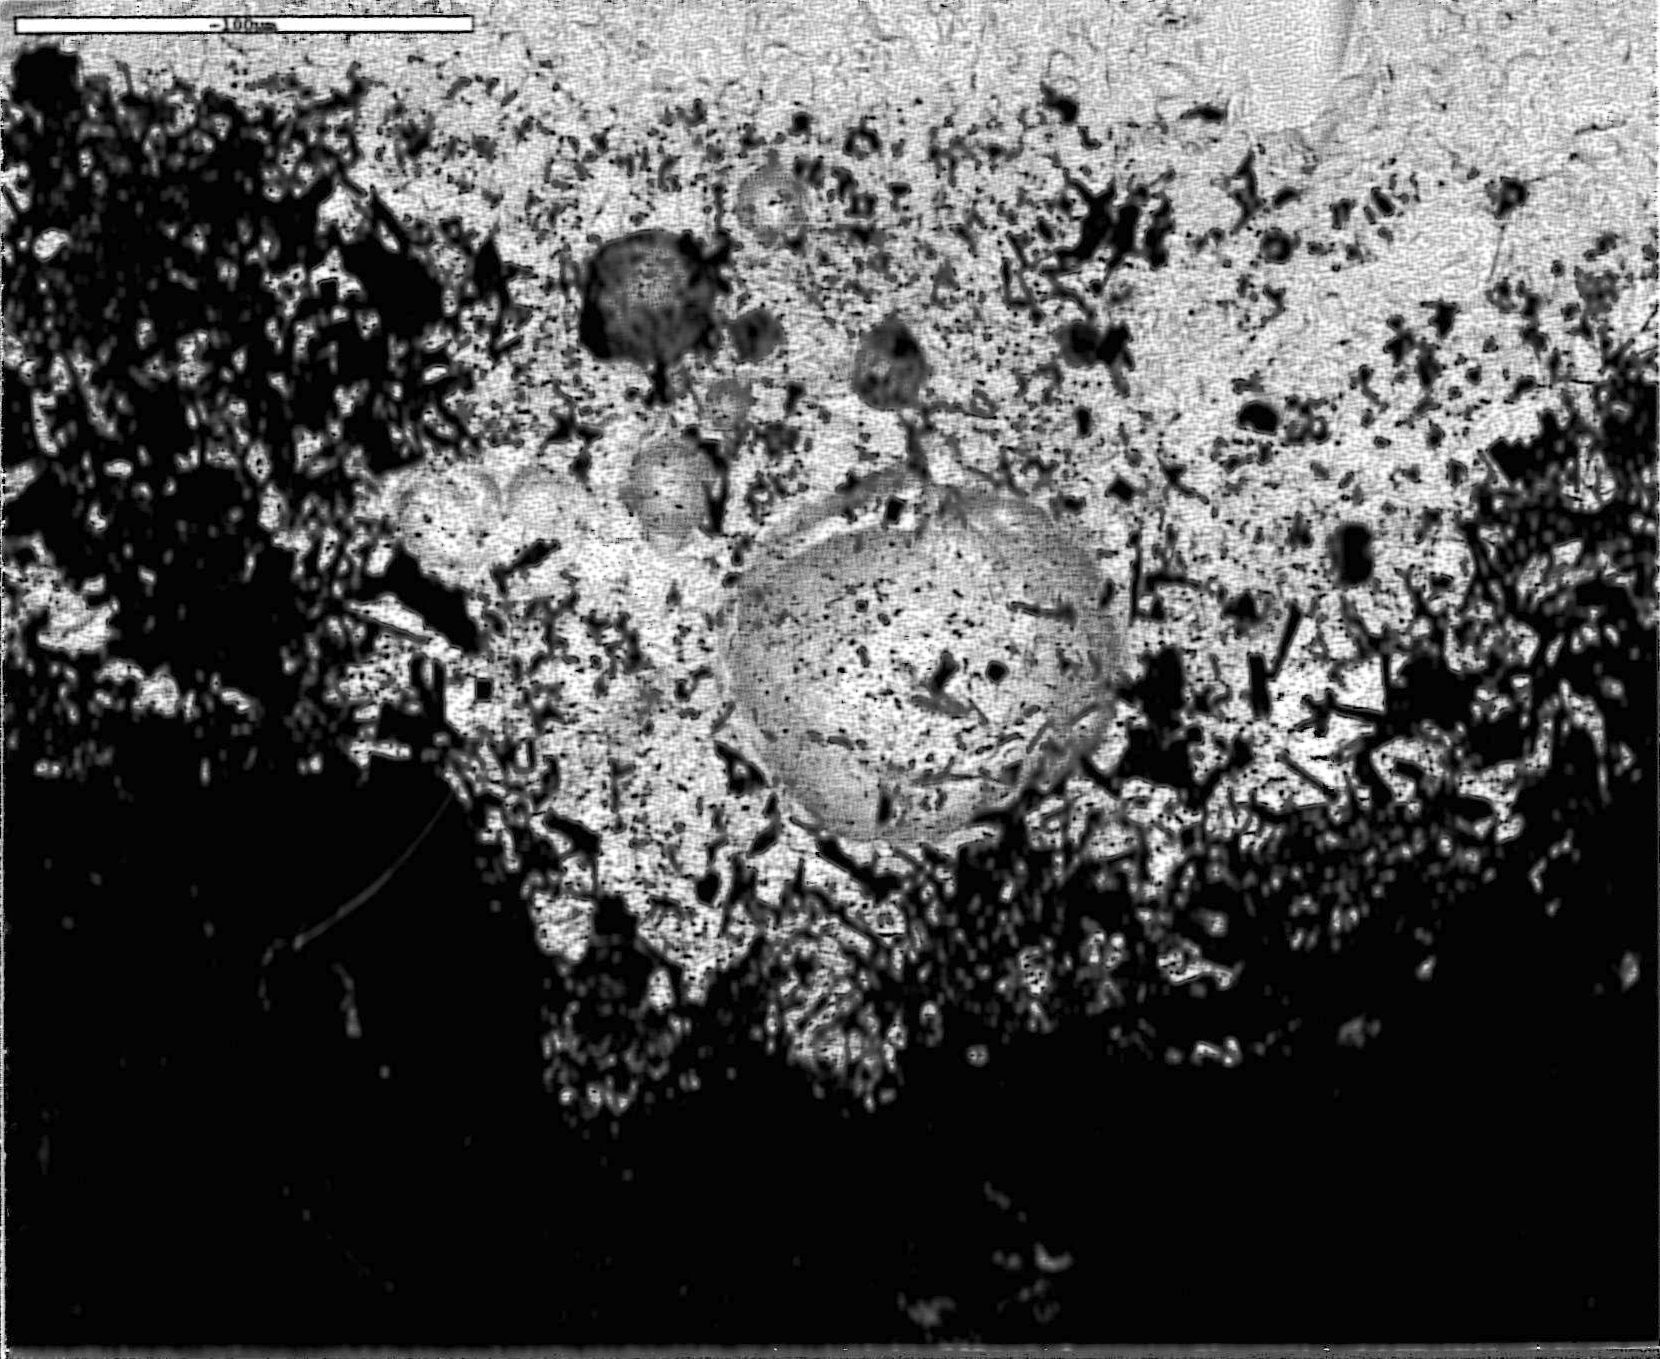
\includegraphics[width=\imgwidth]{PaM_BDX6529_ERD_int}%
    \subcaption{Ensemble glaçure-terre cuite. 
                La barre d'échelle mesure \SI{1}{\mm} 
                (\zone{2.4x1.9}{\mm}) \label{MEB:6529_img_int}}
  \end{minipage}
  \caption[bdx{6529}\ -- Observation de la texture au \MEB, en mode \ERD]
          {\legendeB.
           Observation de la texture au \MEB, en mode \ERD%
          }
  \label{MEB:6529}
\end{figure}

Une \carto de \RX (\fref{MEB:6529_carto_tcgla}) a permis de montrer 
que ces cristaux sont des quartz (\quartz). Ils sont responsables 
des luminescences mauves détectées en \CL.

Des cristaux de forme aciculaire se développent à l'interface 
glaçure-terre cuite (\fref{MEB:6529_img_int}). Cette zone semble être 
riche en potassium, aluminium, calcium, mais plus pauvre en plomb que 
la glaçure environnante.

Le développement important de cette zone d'interface laisse supposer 
des interactions fortes entre glaçure et terre cuite, et donc, 
probablement, une application de la glaçure sur le support céramique 
avant cuisson de ce dernier.

Une \carto de la terre cuite (\fref{MEB:6529_carto_tc}) a permis de 
mettre en évidence la présence de cristaux de quartz et de feldspaths 
potassiques. Ces derniers sont à l'origine des luminescences 
ponctuelles bleues observées en \CL. Les luminescences rouges 
détectées en \CL peuvent être corrélées avec la présence dans la terre 
cuite de calcium, probablement sous forme de calcite (\calcite).

\begin{figure}[htb]
  \includegraphics[width=\textwidth]{PaM_BDX6529_carto}%
  \caption[\bdx{6529}\ -- Observation de la texture au \MEB, \carto 
           de \RX de l'ensemble glaçure-terre cuite]
          {\legendeB.
           Observation de la texture au \MEB, \carto de \RX de 
           l'ensemble glaçure-terre cuite (Gr=90, \zone{1.2x1}{\mm}).}
  \label{MEB:6529_carto_tcgla}
\end{figure}

\begin{figure}[htb]
  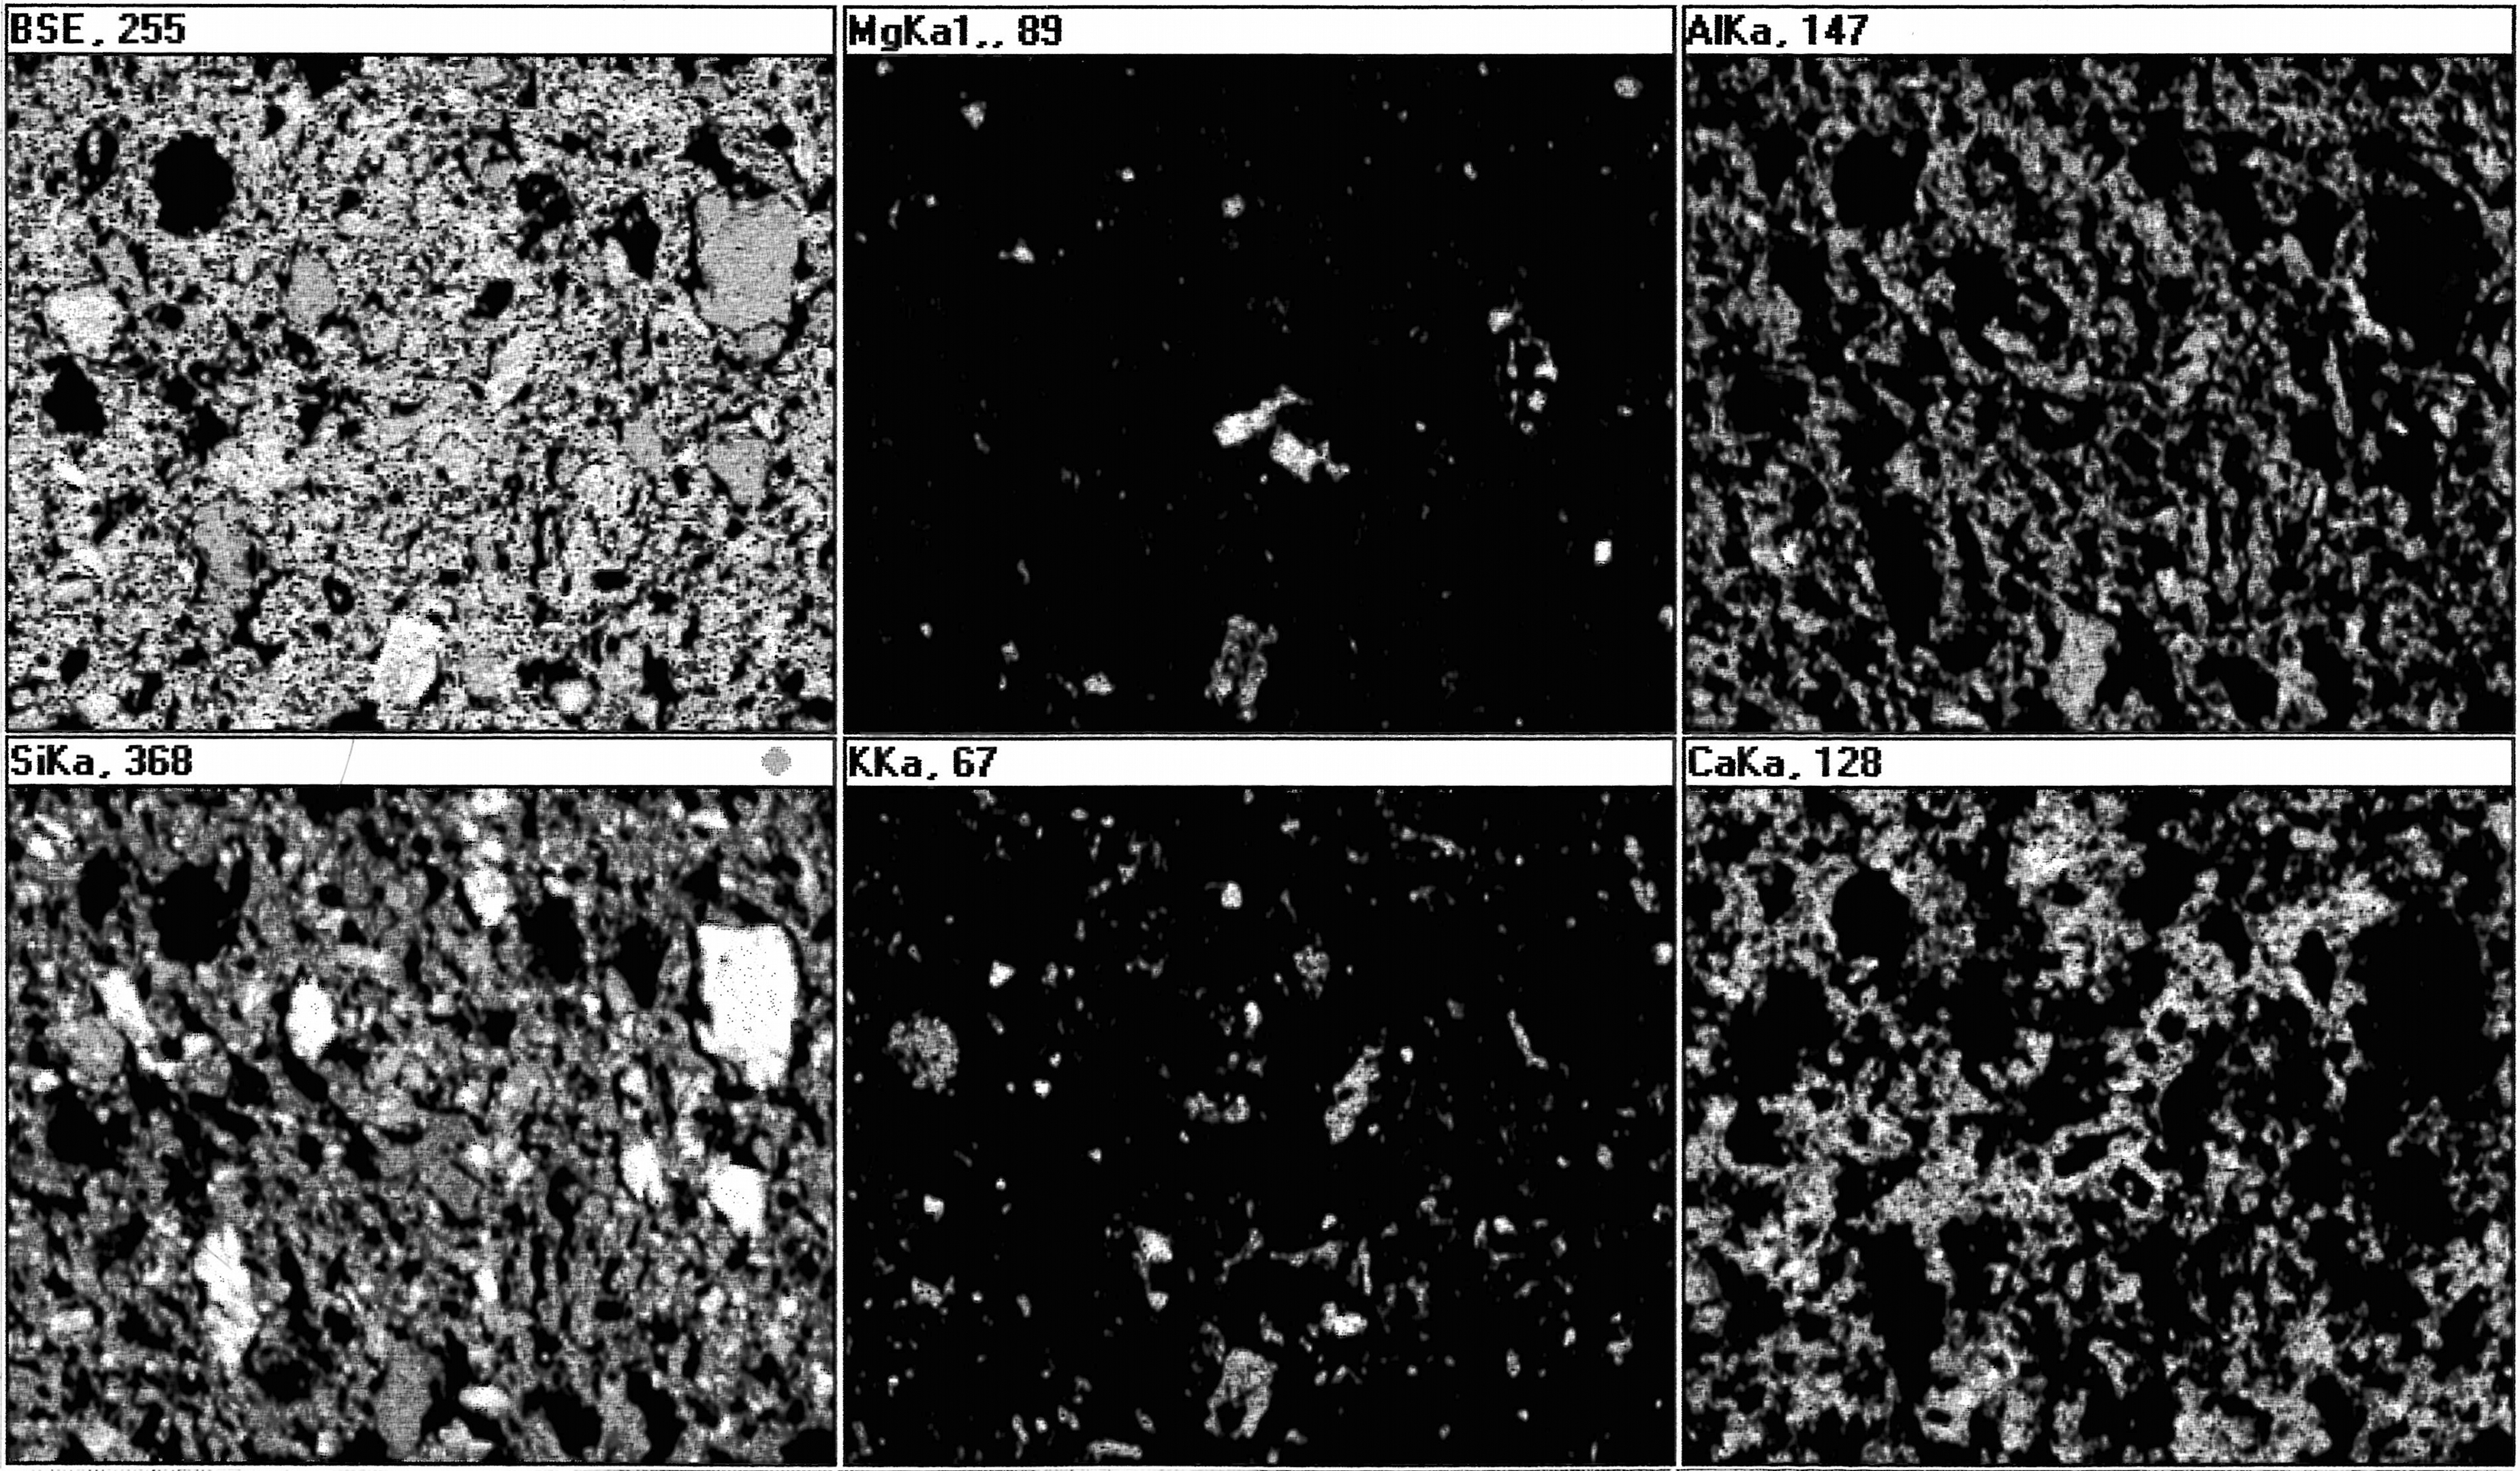
\includegraphics[width=\textwidth]{PaM_BDX6529_carto_tc}%
  \caption[\bdx{6529}\ -- Observation de la texture au \MEB, \carto 
           de \RX de la terre cuite]
          {\legendeB.
           Observation de la texture au \MEB, \carto de \RX de la 
           terre cuite (Gr=200, \zone{550x450}{\um}).}
  \label{MEB:6529_carto_tc}
\end{figure}


\section{Composition élémentaire de la glaçure}
%----------------------------------------------------------------------

\begin{table}[hbt]
  \caption[\bdx{6529}\ -- Analyse quantitative par \EDS, 
           composition élémentaire de la glaçure]
          {\legendeB. Analyse quantitative par \EDS. 
           Composition élémentaire de la glaçure bleue 
           sur une surface de \SI{54x44}{\um} (\PMO).}
  \label{compelem:6529_gla}
  \begin{cartotab}
      \cartolgn{SiO2}{34.02}{1.03} &
      \cartolgn{CaO}{1.95}{0.24} &
      \cartolgn{Al2O3}{0.35}{0.08} &
      \cartolgn{MgO}{0.39}{0.06} 
    \tabularnewline
      \cartolgn{Na2O}{0.50}{0.08} &
      \cartolgn{K2O}{1.56}{0.12} &
      \cartolgn{Fe2O3}{0.55}{0.13} &
      \cartolgn{PbO}{56.75}{1.46} 
    \tabularnewline
      \cartolgn{SnO2}{2.39}{0.24} &
      \cartolgnnd{CuO} &
      \cartolgnnd{CoO} &
      \cartolgnnd{MnO}
    \tabularnewline
      \cartolgnnd{Cr2O3} &
      \cartolgnnd{ZnO} &
      \cartolgnnd{Sb2O3} &
      \cartolgnnd{TiO2}
    \tabularnewline
      \cartolgn{S}{0.34}{0.05} &
      \cartolgn{P2O5}{0.70}{0.13} &
      \cartolgn{Cl}{0.51}{0.06} &
      \cartolgnnd{As2O3}
    \tabularnewline
  \end{cartotab}
\end{table}

La glaçure est plombifère et opacifiée à l'étain 
(\fref{compelem:6529_gla}). Le cobalt, responsable de la 
coloration bleue (mis en évidence par \SAO), n'est pas détecté. 
Il est probablement présent en concentration inférieure au seuil 
de détection de la méthode. Il possède en effet un très fort pouvoir 
colorant : \SI{0.25}{\percent} de cobalt suffisent à donner un bleu 
moyen \autocite{Rhodes_1999}.


\section{Étude de la terre cuite support}
%----------------------------------------------------------------------

\subsection{Composition élémentaire}
%~~~~~~~~~~~~~~~~~~~~~~~~~~~~~~~~~~~~~~~~~~~~~~~~~~~~~~~~~~~~~~~~~~~~~~
\begin{table}[hbt]
  \caption[\bdx{6529}\ -- Analyse quantitative par \EDS, 
           composition élémentaire de la terre cuite]
          {\legendeB. Analyse quantitative par \EDS. 
           Composition élémentaire de la terre cuite 
           sur une surface de \SI{1080x876}{\um} (\PMO)}
  \label{compelem:6529_tc}
  \begin{cartotab}
      \cartolgn{SiO2}{49.38}{0.61} &
      \cartolgn{CaO}{18.70}{0.88} &
      \cartolgn{Al2O3}{14.97}{0.33} &
      \cartolgn{MgO}{2.50}{0.35} 
    \tabularnewline
      \cartolgn{Na2O}{0.62}{0.07} &
      \cartolgn{K2O}{2.26}{0.21} &
      \cartolgn{Fe2O3}{9.06}{0.18} &
      \cartolgnnd{PbO}
    \tabularnewline
      \cartolgnnd{SnO2} &
      \cartolgnnd{CuO} &
      \cartolgnnd{CoO} &
      \cartolgnnd{MnO}
    \tabularnewline
      \cartolgnnd{Cr2O3} &
      \cartolgnnd{ZnO} &
      \cartolgnnd{Sb2O3} &
      \cartolgn{TiO2}{0.85}{0.03}
    \tabularnewline
      \cartolgnnd{S} &
      \cartolgn{P2O5}{1.59}{0.15} &
      \cartolgn{Cl}{0.07}{0.01} &
      \cartolgnnd{As2O3}
    \tabularnewline
  \end{cartotab}
\end{table}

La terre cuite est de type calcique (\SI{18.70}{\percent} de CaO). 
Sa coloration ocre rose est due au \ch{Fe^3+} en atmosphère de cuisson 
oxydante \autocite{Echallier_1984}.

\subsection{Composition \cristallo}
%~~~~~~~~~~~~~~~~~~~~~~~~~~~~~~~~~~~~~~~~~~~~~~~~~~~~~~~~~~~~~~~~~~~~~~
Le principal composé cristallisé mis en évidence par \DX sur poudre 
(\fref{DRX:6529}) est le quartz (\quartz). On relève également la 
présence, à des teneurs plus faibles, de calcite (\calcite) pouvant 
correspondre aux émissions rouges détectées en \CL, d'albite (\albite), 
de diopside alumineux (\diopsideal) et de gehlénite (\gehlenite). 
Ces deux derniers cristaux peuvent être responsables des émissions 
bleues détectées en \CL.

La présence de diopside alumineux et de gehlénite, deux phases se 
développant à haute température, associées à l'albite, disparaissant 
vers \SI{900}{\degC} au profit de l'anorthite, laisse penser que la 
température de cuisson de la céramique se situe autour de 
\SIrange{850}{900}{\degC} \autocite{Peters_1978}.

\begin{figure}[htb]
  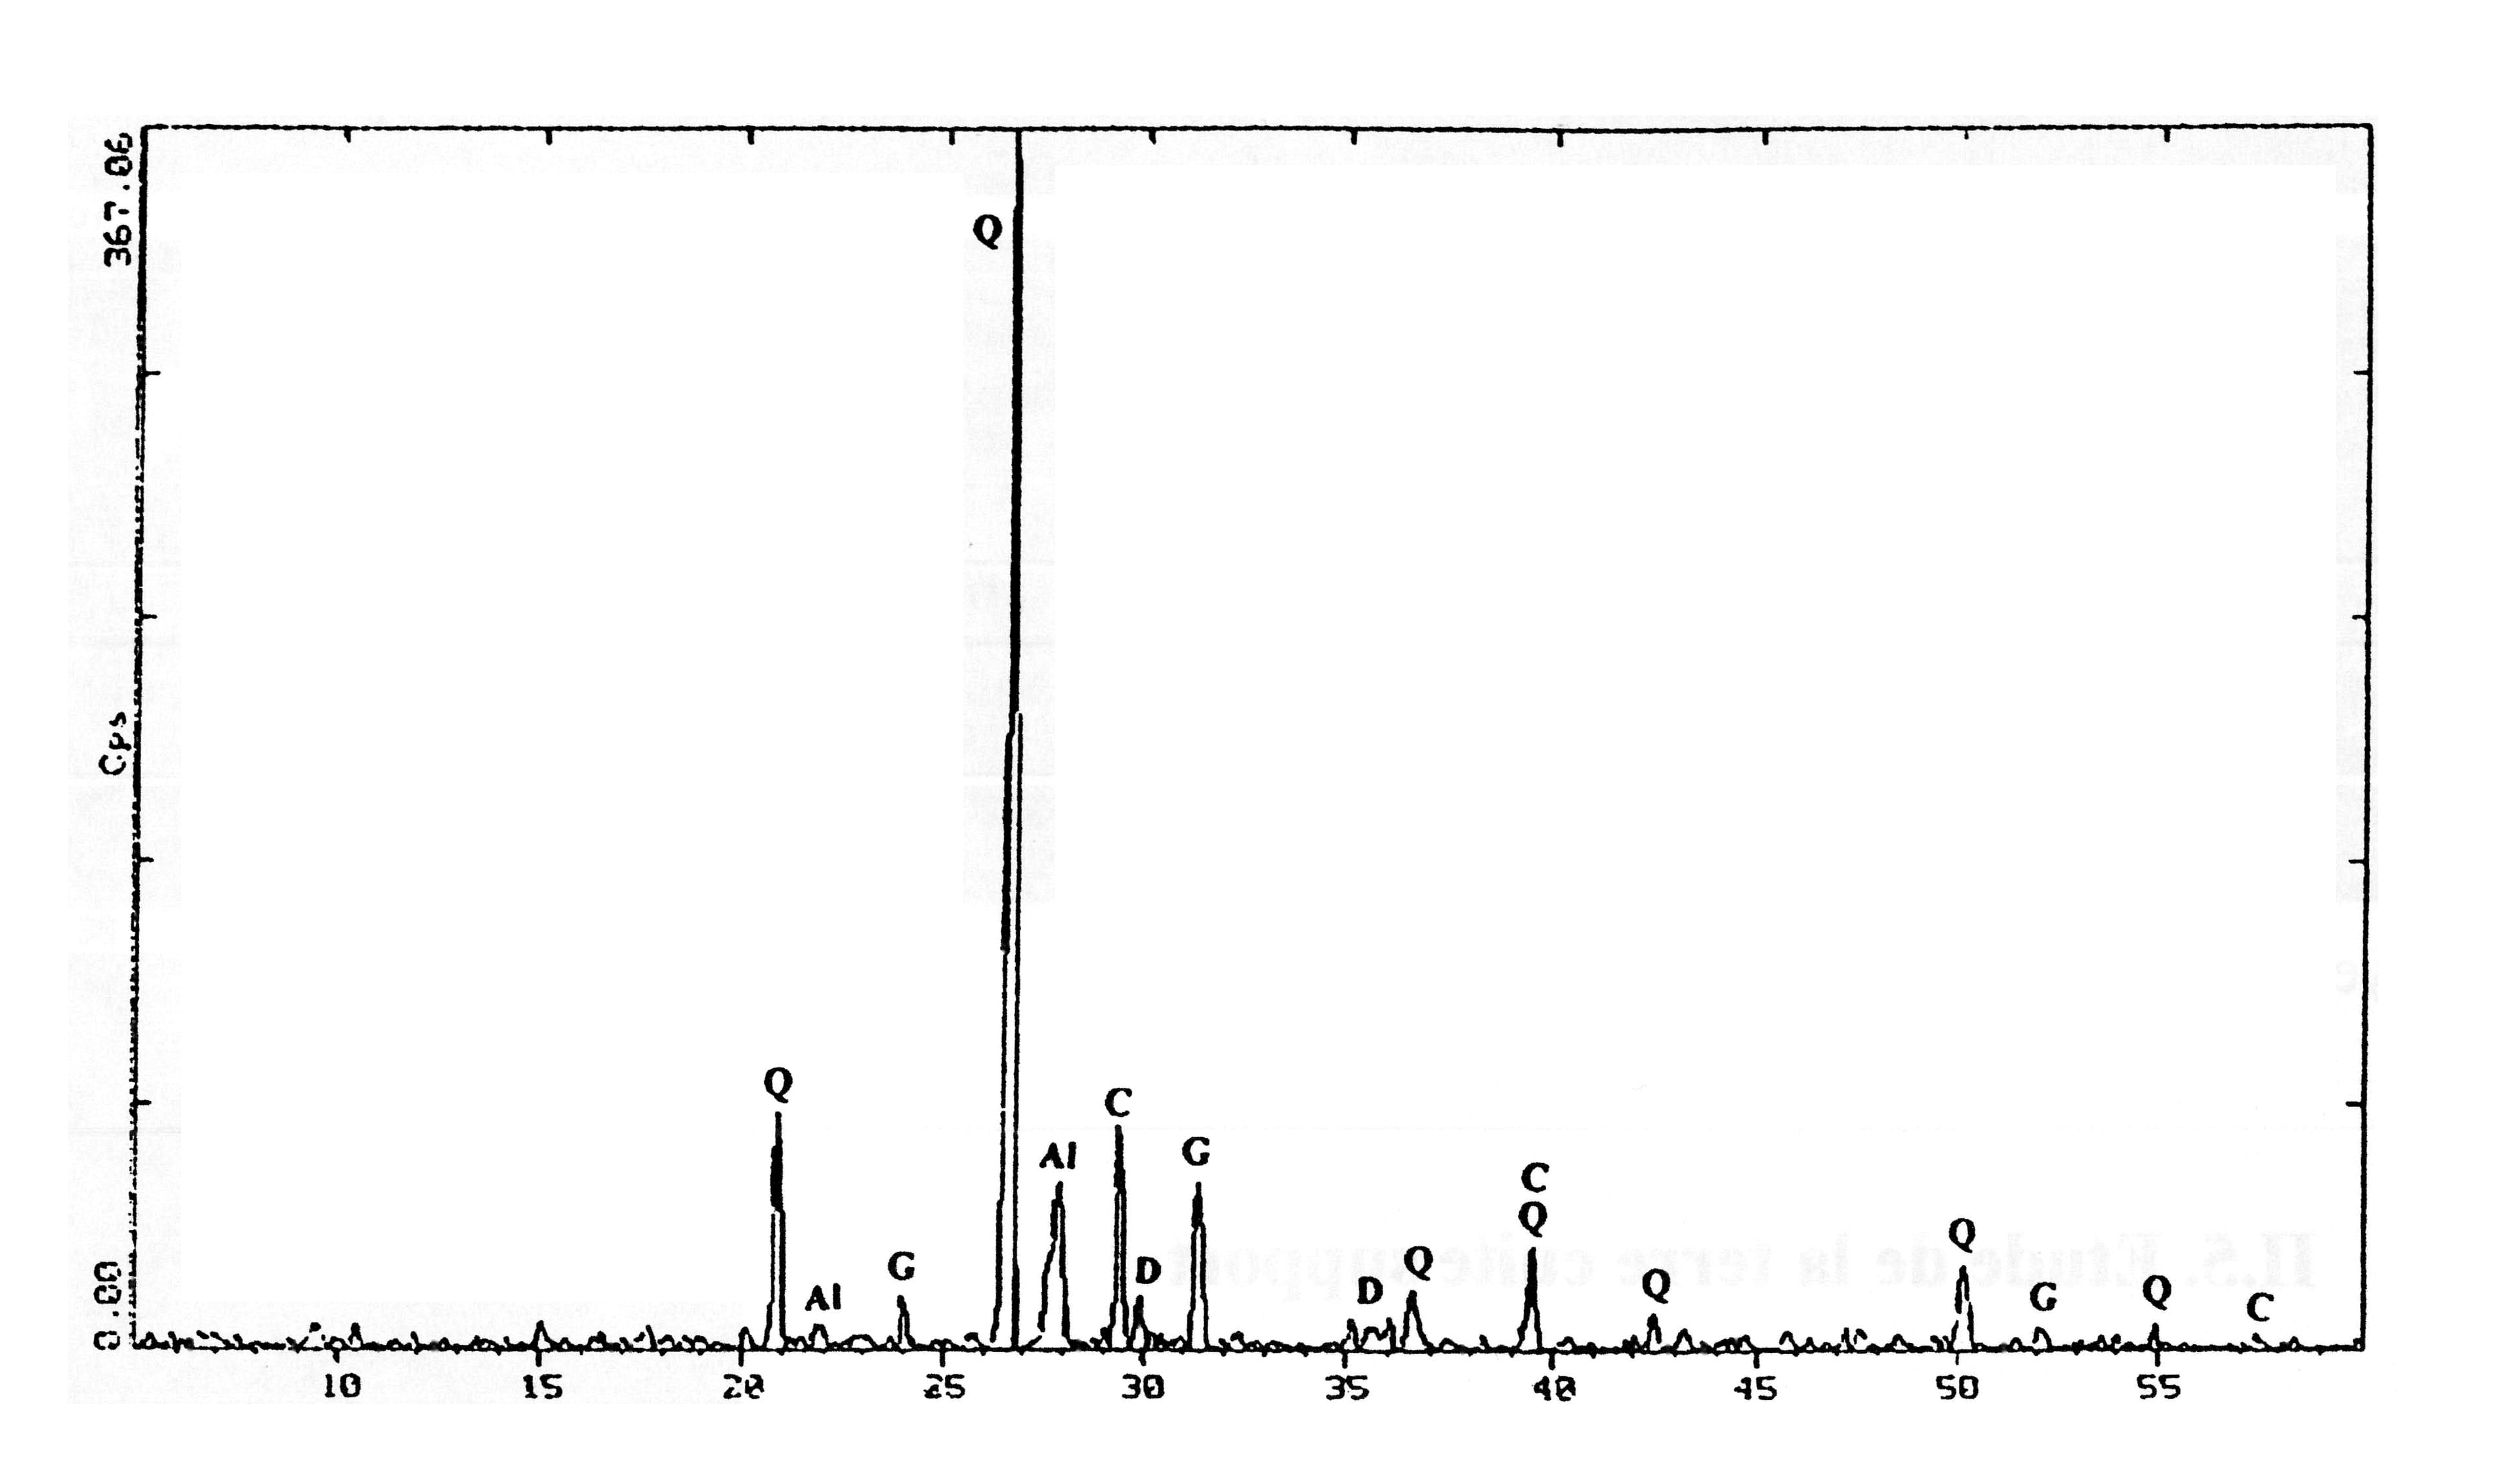
\includegraphics[width=\textwidth]{PaM_BDX6529_DX}
  \caption[\bdx{6529}\ -- Diffraction de \RX sur poudre 
           de la terre cuite]
          {\legendeB.
           \DX[D] sur poudre de la terre cuite. 
           Mise en évidence de la présence de quartz (Q), 
           calcite (C), albite (Al), gehlénite (G), diopside (D).}
  \label{DRX:6529}
\end{figure}


\section{Sur la présence et l'identification de cristaux de 
         dévitrification}
%----------------------------------------------------------------------

On distingue, dans la zone d'interface terre cuite-glaçure, des 
cristaux de forme aciculaire (\fref{MEB:6529_img_cx}). Ce sont 
des cristaux de dévitrification qui se développent pendant le 
refroidissement lent du matériau, à partir de germes se formant à 
haute température. Des analyses ponctuelles (\tref{compelem:6529_cx}) 
ont montré qu'il s'agit d'alumino-silicates mixtes de potassium, de 
calcium et de plomb que l'on peut appeler des \frquote{feldspaths de 
plomb}.

\begin{figure}[htb]
  \setlength{\imgwidth}{7cm}
  \setlength{\mylength}{1cm+\imgwidth}
  \setlength{\sidecapwidth}{\linewidth-\sidecapsep-\mylength-1cm}
  \renewcommand*{\sidecapfloatwidth}{\mylength}%
  \sidecapmargin{left}%
  \RaggedLeft
  \begin{sidecaption}[%
    \bdx{6529}\ -- Image en mode \ERD, 
    cristaux de dévitrification de forme aciculaire%
  ]{%
    \legendeB.
    Observation au \MEB, image en mode \ERD. 
    Cristaux de dévitrification de forme aciculaire. La barre 
    d'échelle mesure \SI{20}{\um} (\zone{70x55}{\um}).%
  }[MEB:6529_img_cx]
    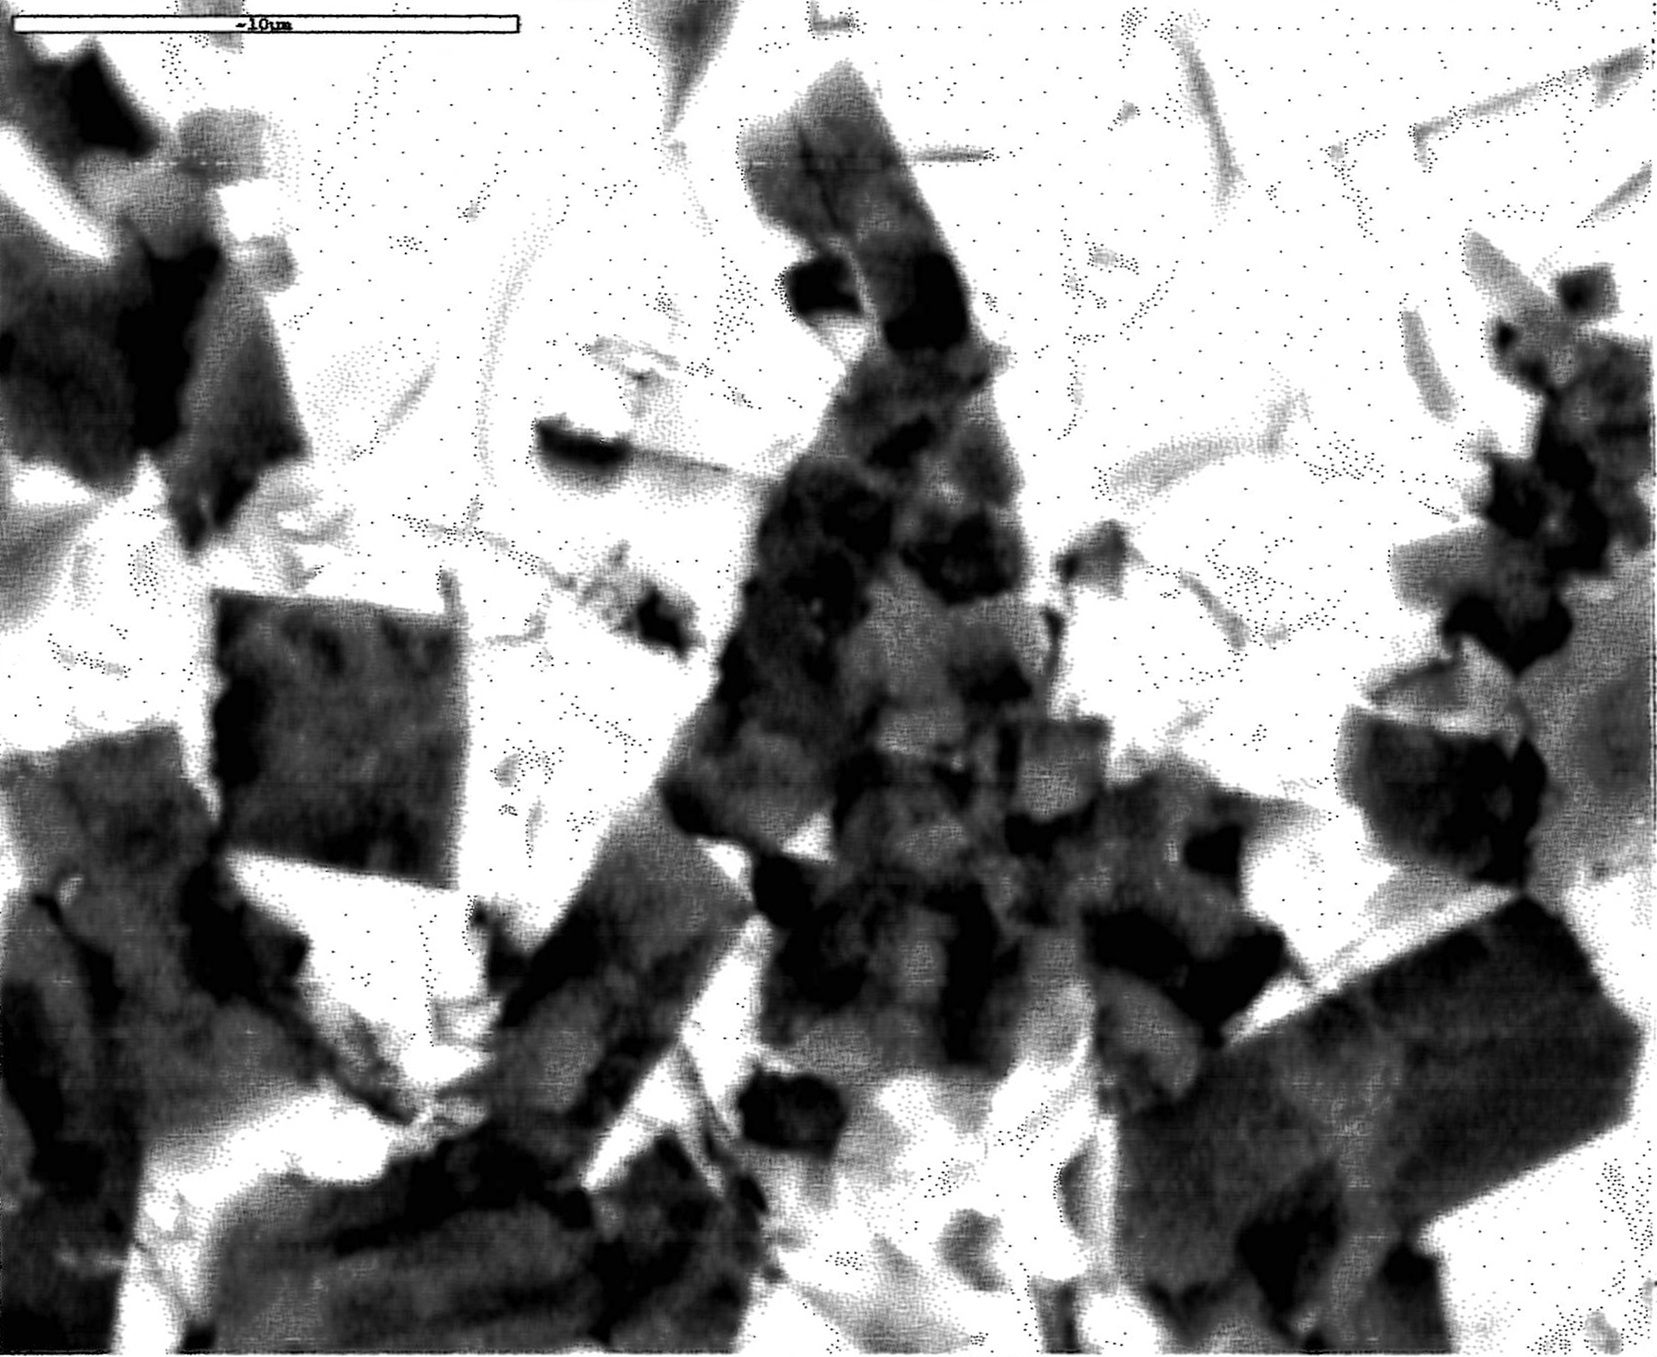
\includegraphics[width=\imgwidth]{PaM_BDX6528_ERD_cx}%
  \end{sidecaption}
\end{figure}


\begin{table}[hbt]
  \caption[\bdx{6529}\ -- Analyse quantitative par \EDS, 
           composition élémentaire des cristaux de dévitrification]
          {\legendeB. Analyse quantitative par \EDS. 
           Composition élémentaire des cristaux de dévitrification 
           par analyses ponctuelles (\SI{1}{\um\squared}) (\PMO).}
  \label{compelem:6529_cx}
  \begin{cartotab}
      \cartolgn{SiO2}{54.61}{6.48}  &
      \cartolgn{CaO}{3.51}{1.64}    &
      \cartolgn{Al2O3}{11.80}{2.82} &
      \cartolgn{MgO}{0.28}{0.13}
    \tabularnewline
      \cartolgn{Na2O}{1.06}{0.13}  &
      \cartolgn{K2O}{9.44}{2.19}   &
      \cartolgn{Fe2O3}{2.09}{0.32} &
      \cartolgn{PbO}{16.83}{10.17}
    \tabularnewline
      \cartolgnnd{SnO2} &
      \cartolgnnd{CuO}  &
      \cartolgnnd{CoO}  &
      \cartolgnnd{MnO}
    \tabularnewline
      \cartolgnnd{Cr2O3} &
      \cartolgnnd{ZnO}   &
      \cartolgnnd{Sb2O3} &
      \cartolgn{TiO2}{0.14}{0.09}
    \tabularnewline
      \cartolgnnd{S}            &
      \cartolgnnd{P2O5}         &
      \cartolgn{Cl}{0.24}{0.15} &
      \cartolgnnd{As2O3}
    \tabularnewline
  \end{cartotab}
\end{table}


\section{Étude des altérations de la glaçure}
%----------------------------------------------------------------------

Aucune figure d'altération n'a été mise en évidence dans la glaçure, 
ni visuellement, ni en \MEB[ie] (MEB).


\section{Bilan}
%----------------------------------------------------------------------

Cet échantillon est donc une pièce de céramique portant une glaçure 
plombifère dont la coloration bleue est due au \ch{Co^2+} en 
atmosphère de cuisson oxydante et légèrement opacifiée à l'étain pour 
rendre la couleur plus veloutée et masquer la terre cuite rougeâtre.

Son support de terre cuite est de type calcique. Sa coloration 
rougeâtre est due à la présence de \ch{Fe^3+} en atmosphère de 
cuisson oxydante.

Sa composition \cristallo (quartz, calcite, albite, diopside, 
gehlénite) laisse penser qu'elle a été cuite à une température 
de l'ordre de \SIrange[range-phrase=\ à\ ]{850}{900}{\degC}.

À l'interface glaçure-terre cuite, on distingue un large liseré 
continu présentant une luminescence jaune, associé à la présence de 
cristaux de dévitrification identifiés comme des alumino-silicates 
mixtes de potassium, de calcium et de plomb (ou \frquote{feldspaths 
de plomb}). Le développement important de cette zone laisse penser à
une application de la glaçure sur la terre crue.

La glaçure ne présente pas de figure d'altération d'origine chimique 
mais une usure mécanique de surface.
